%!TEX root = ../chapter1.tex
%******************************
%	 Results 
%*****************************

\section{scRNAseq of murine CD4$^+$ T cells}
\subsection*{Single-cell RNA sequencing of CD4$^+$ T cells during activation, ageing and across two mouse species}

\begin{wrapfigure}{r}{0.5\textwidth}
\centering    
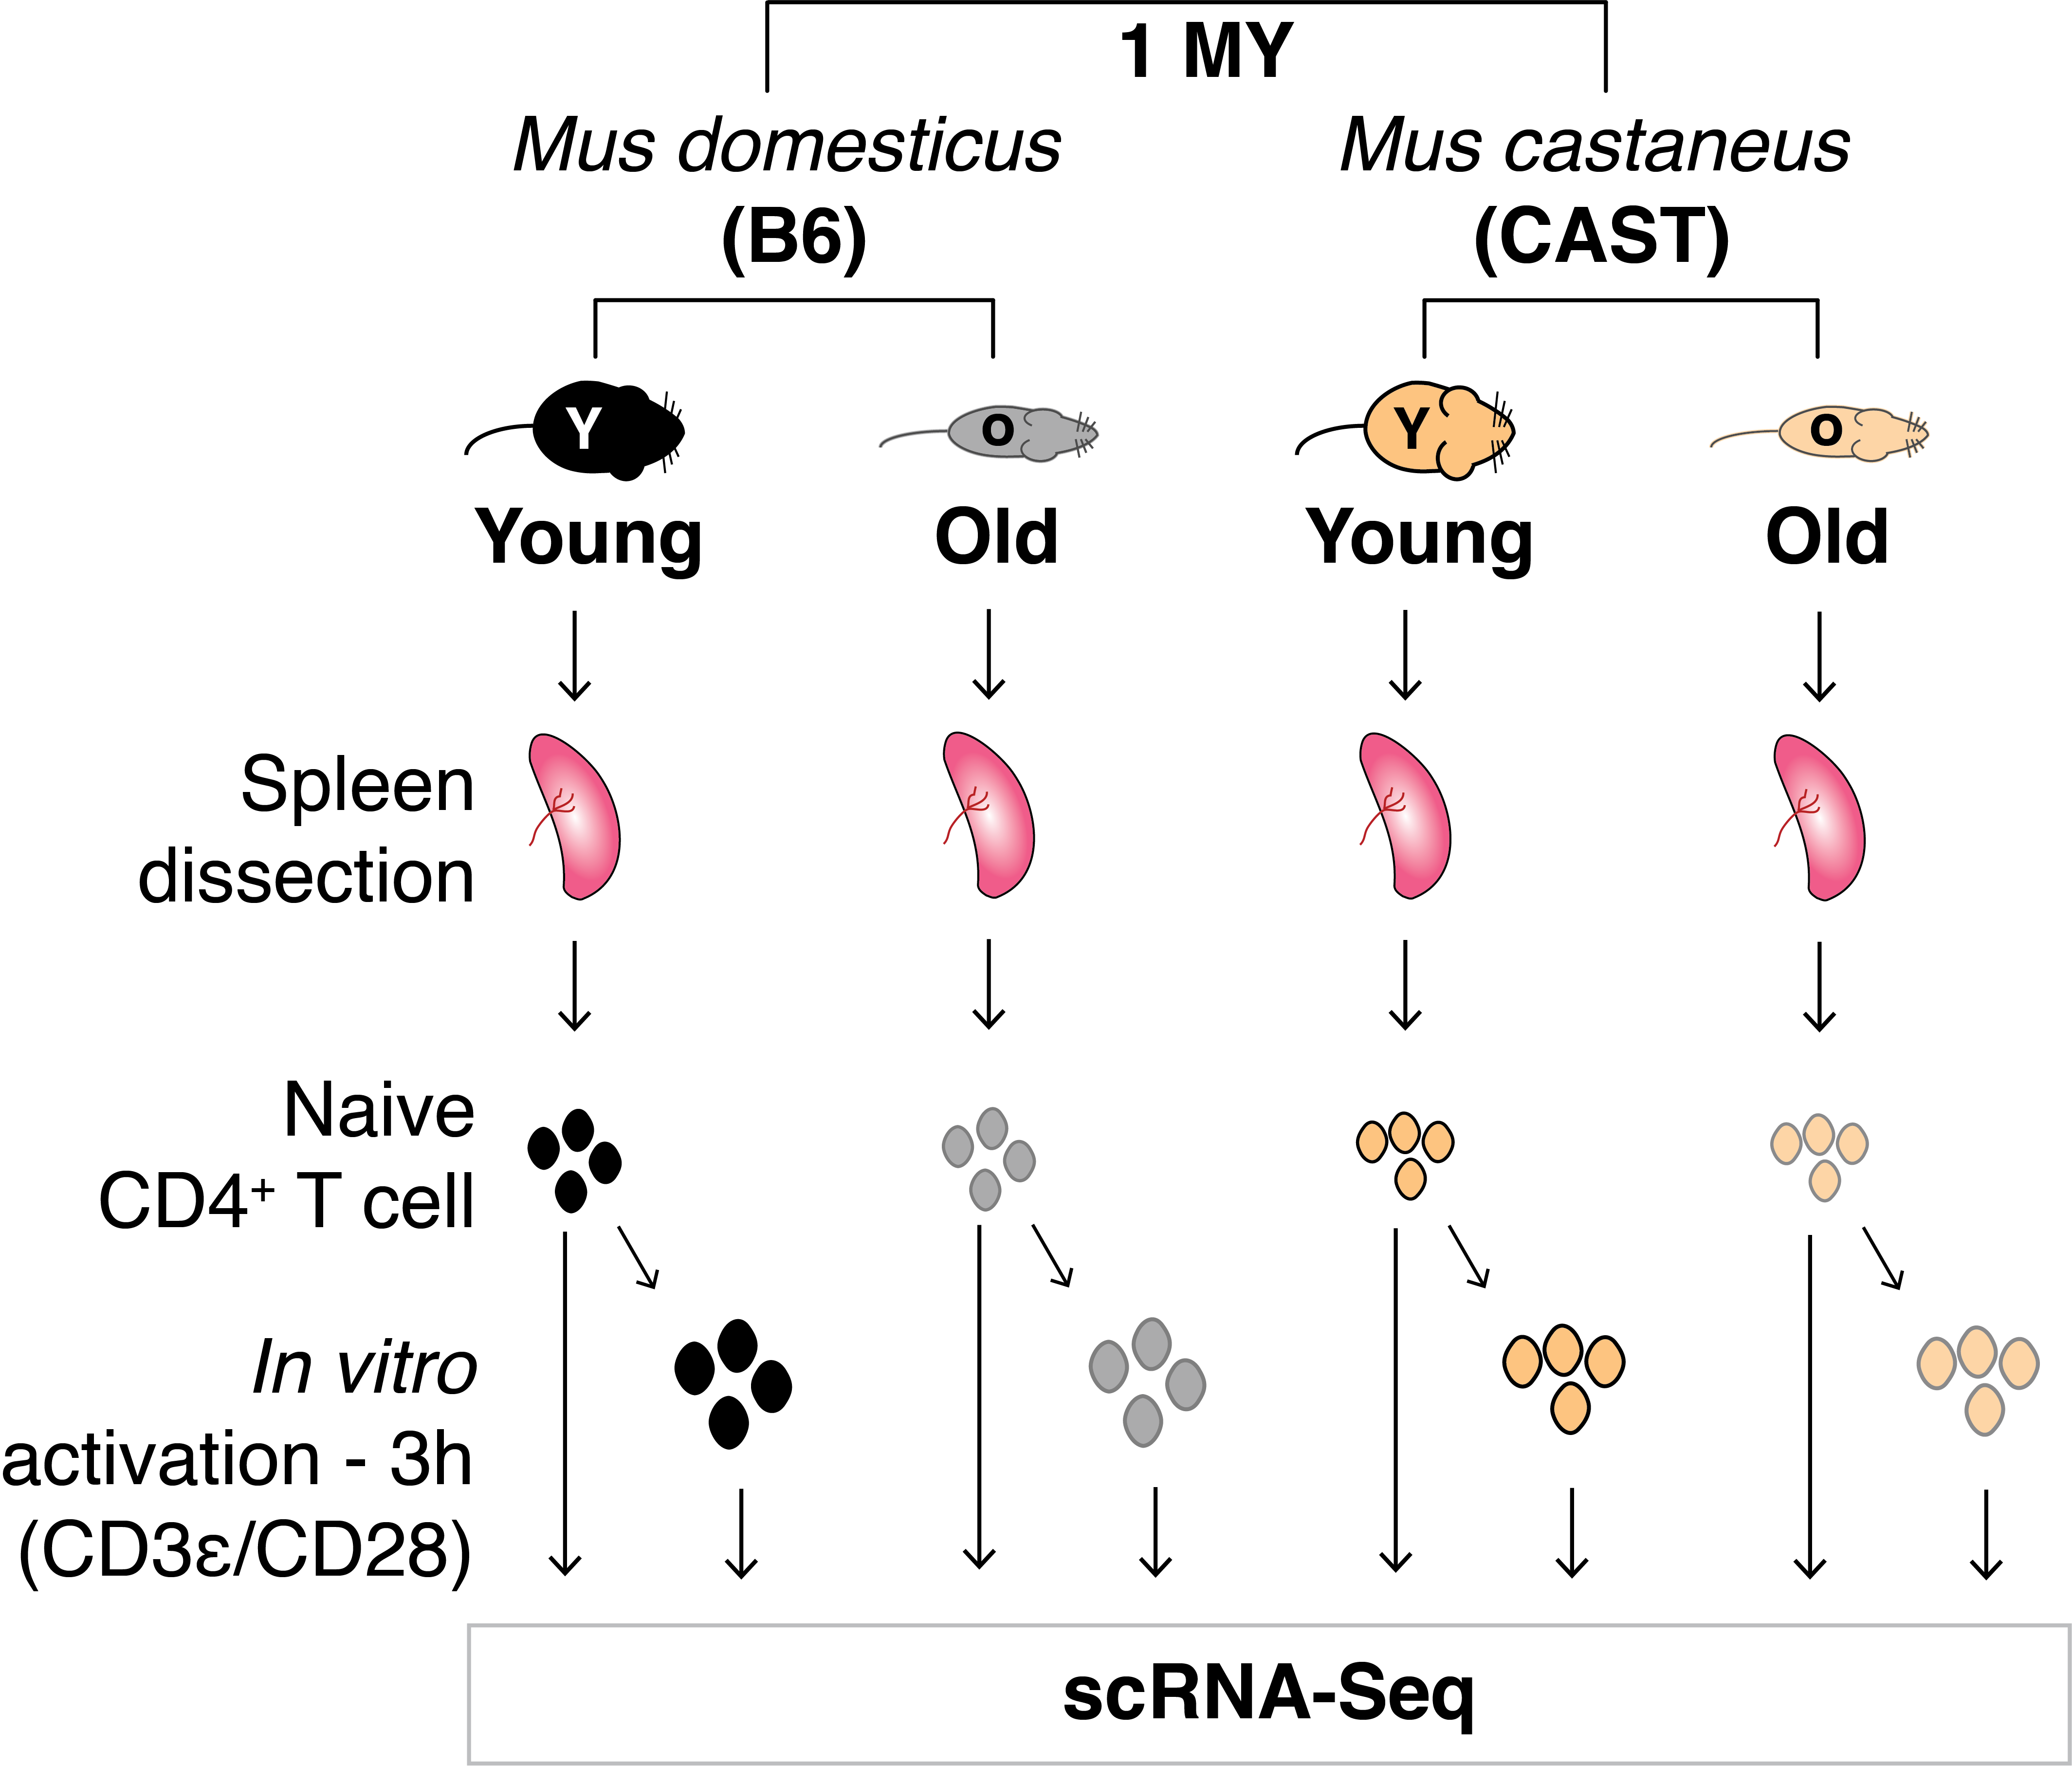
\includegraphics[width=0.48\textwidth]{Fig_1.png}
\caption[scRNAseq of CD4$^+$ T cells from young and old mice.]{\textbf{scRNAseq of unstimulated and activated CD4$^+$ T cells from young and old B6 and CAST animals.} \\
Single cells were isolated from spleens of young (~3 month) and old (~21 month) individuals of two related mouse sub-species (Mus musculus domesticus, B6; Mus musculus castaneus, CAST). Isolated cells were subjected to single-cell mRNA sequencing (scRNAseq) before or after 3 hours of in vitro activation using anti-CD3$\epsilon$/CD28 coated plates.}
\label{fig:chapt1_overview}
\end{wrapfigure}

To assess the conservation of immune activation programmes, we isolated CD4$^+$ T cells from healthy individuals of two inbred mouse sub-species separated by 1 million years of divergence: the reference C57BL/6J, Mus musculus domesticus (B6); CAST/EiJ, Mus musculus castaneus (CAST)). We characterized their gene expression programmes by single-cell RNA-sequencing (scRNAseq) during ageing in young (~3 months) and old (~21 months) individuals of each strain \textbf{(Fig. \ref{fig1:chapt1_overview})}. These two sub-species have similar lifespans \citep{Yuan2011}, and CAST mice showed the hallmarks of normal organismal aging observed in B6 mice \citep{Rodwell2004}. All mice were healthy at the time of experiments. To asses different CD4$^+$ T cell compartments, we assayed cell populations with different levels of purity. First, we isolated all unstimulated CD4$^+$ T cells from spleen of old and young animals. Secondly, we highly purified naive CD4$^+$ T cells and effector memory (EM) CD4$^+$ T cells. For each species/condition, scRNA-seq experiments were performed using cells isolated from two individual mice.

\subsubsection*{Unstimualted CD4$^+$ T cells}

Unstimulated naive CD4$^+$ T cells were purified from dissociated mouse spleens using cell strainers, cell separation media and a MACS CD4$^+$ CD62L$^+$ T Cell Isolation Kit. Purified naive CD4$^+$ T cells were cultured in IMDM medium supplemented with 10\% Fetal Bovine Serum, 1 $\mu$g/mL Penicillin/Streptomicin, and 50 $\mu$M 2-mercaptoethanol. \\

\subsubsection{Naive and effector memory CD4$^+$ T cells}

\begin{wrapfigure}{r}{0.5\textwidth}
\centering    
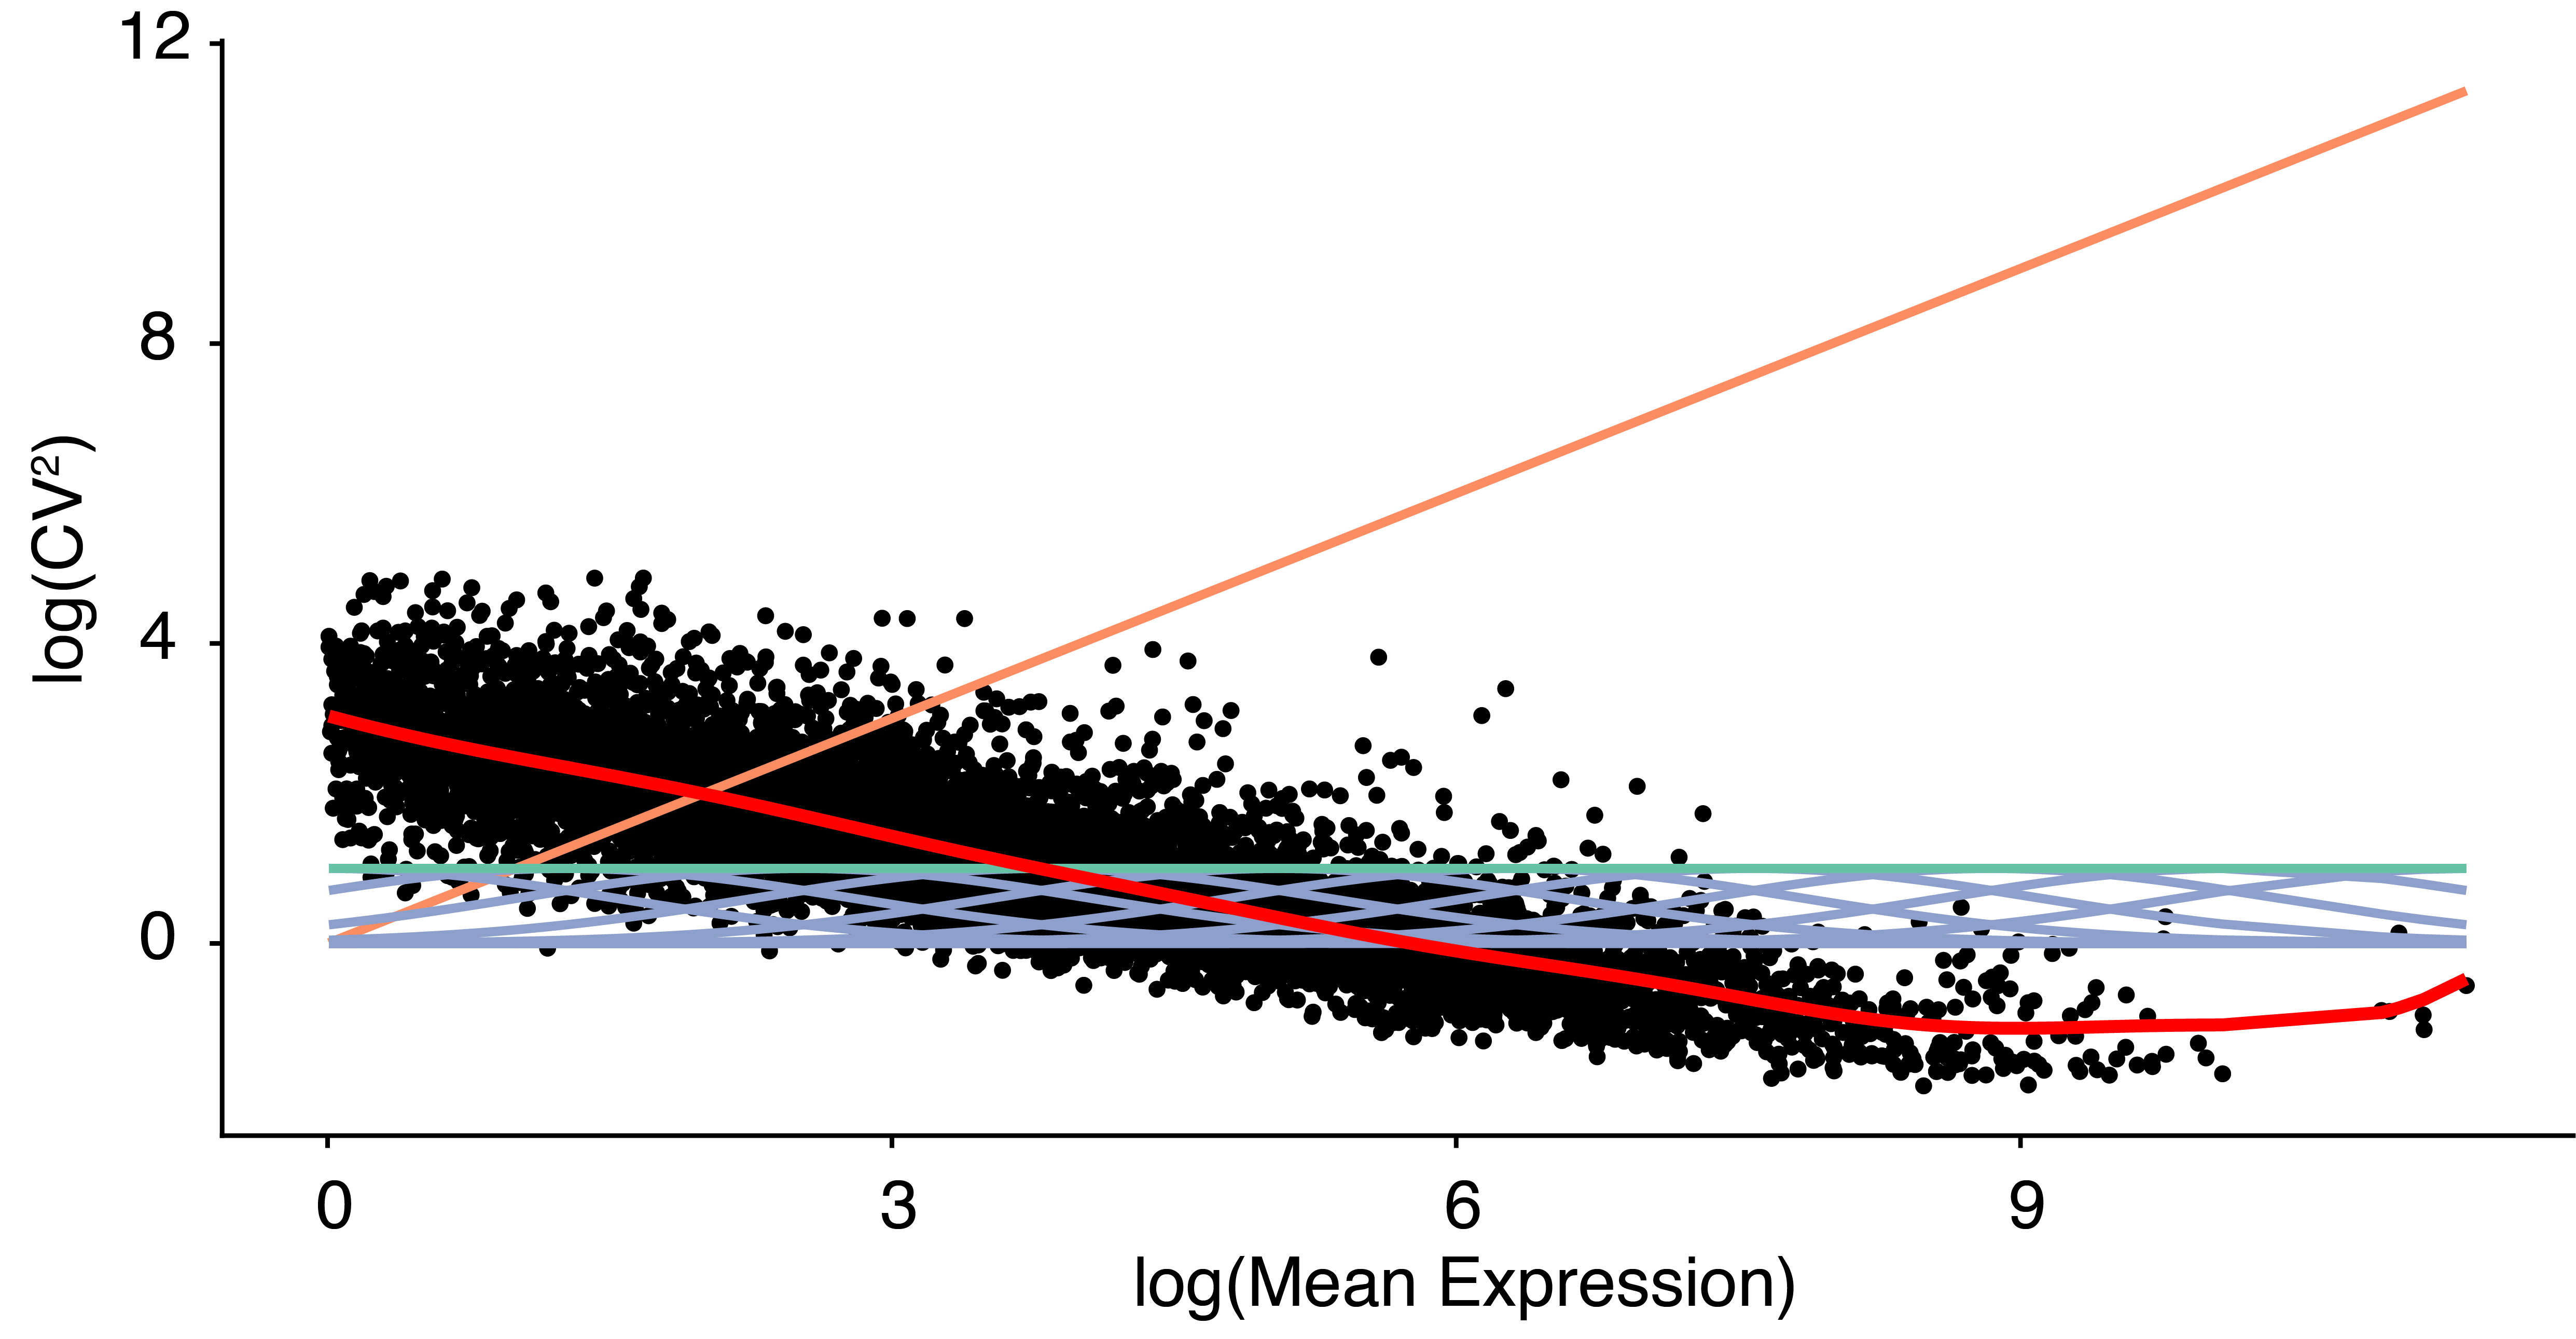
\includegraphics[width=0.48\textwidth]{Fig_2.png}
\caption[FACS of naive and effector memory CD4$^+$ T cells.]{\textbf{FACS of naive and effector mempry CD4$^+$ T cells.} \\
Gating Strategy: lymphocytes were gated by the use of forward scatter (FSC-A) and side scatter (SSC-A). Cell doublets were excluded according to area and height of forward scatter (FSC-A/FSC-H). Dead cells were removed using viability dye. PD-1$^+$ CD4$^+$ T cells were excluded and PD-1-ve CD4$^+$ T cells were further separated into naive and EM CD4$^+$ T cell subsets according to their CD44 and CD62L expression. Cells with a mature CD24lo Qa2hi phenotype were then gated from naive and EM subsets and CD69+ cells were removed.}
\label{fig1:FACS}
\vspace*{-20mm}
\end{wrapfigure}

Naive and effector memory CD4$^+$ T cells were purified from spleens of both young and old C57/BL6 mice by FACS.  Briefly, spleens were harvested from both young and old animals and single cell suspensions were obtained by meshing through a cell strainer (70 $\mu$m). B cells were depleted from cell suspensions by MACS using CD19 microbeads and red blood cells were lysed with RBC lysis buffer. The enriched cell fraction was then stained with Fixable eFluor 780 viability dye following by Fc receptor blocking with TruStain fcXTM and subsequent staining with a panel of fluorescence-conjugated antibodies against CD4, CD44, CD62L, CD24, Qa2, CD69 and PD-1.  Stained cells were immediately sorted using a 5-laser Aria IIu SORP instrument with the stringent gating strategy described in \textbf{Fig. \ref{fig1:FACS}}. \\
Hereafter, for simplification and clarity, purified unstimulated CD4$^+$ T cells will be named naive, stimulated cells will be named activated.

\subsubsection*{Activation of CD4$^+$ T cells}

Naive cells were seeded into 96-well plates coated for 1h at 37ºC with anti-CD3$\epsilon$ (1 $\mu$g/ml) and anti-CD28 (3 $\mu$g/ml) at a density of 80,000-120,000 cells/ml, and then cultured in a total volume of 100 $\mu$l media that did not contain cytokines or additional antibodies.

\subsubsection*{scRNAseq using the Fluidigm C1 system}

Naive, purified naive and activated CD4+ T cells were immediately collected and loaded on a 5–10$\mu$m Auto Prep Integrated Fluidic Circuit (IFC) to capture single cells using the C1 Single cell Auto Prep System (Fluidigm). All IFCs were visually inspected, and wells with multiple cells or cell debris were marked as low quality. Upon cell capture, reverse transcription and cDNA amplification were performed using the SMARTer PCR cDNA Synthesis Kit and the Advantage 2 PCR Kit. ERCC spike-in RNA (1 $\mu$L diluted at 1:50,000) was added to the C1 lysis mix. All capture sites were included for the RNA-seq library preparation.

\subsubsection*{Read alignment to reference genomes}

Read alignment to reference genomes was performed using \emph{gsnap} with default parameters, while supplying splice-site positions. Samples taken from B6 were mapped against the mouse reference GRCm38. CAST samples were aligned against the \emph{Mus musculus castaneus de novo} genome assembly [ftp://ftp-mouse.sanger.ac.uk/REL-1509-Assembly/], which was used under an advance access agreement [ftp://ftp-mouse.sanger.ac.uk/REL-1509-Assembly/README]. Gene annotation for B6 was taken from the GRCm38 reference; gene annotation for CAST was taken from the newly constructed \emph{Mus musculus castaneus} assembly [http://hgwdev.cse.ucsc.edu/$\sim$ifiddes/mouse\_{}genomes\_{}data/, version 0.2]. Additionally, since mitochondrial genes and certain immune genes (e.g., CD28) are absent from the most recent \emph{Mus musculus castaneus} annotation, and since high mitochondrial gene expression is a well-established signature of low-quality single-cell transcriptome profiles \citep{Ilicic2016}, we also mapped CAST reads against GRCm38 and used the B6 annotation solely for these genes. Gene expression counts were obtained using HTSeq with default options. Only genes with orthologs in both species were considered for downstream analysis. 

\subsubsection*{Computational quality control and filtering}

We visually inspected the vast majority of cell-capture sites in each C1 small-integrated fluidic circuit using 40x magnification lensing to ensure precise capture of single cells \textbf{(Fig. \ref{fig1:QC}A and B)}. Low-quality cells were computationally filtered using the following quality control criteria, developed by previous single-cell RNA-sequencing studies \citep{Brennecke2013, Buettner2015, Scialdone2015, Vallejos2015BASiCS}:\\
The percentage of reads mapping to annotated genomic regions was compared to the percentage of reads mapping to ERCC spike-ins. Cells with low genomic read (< 20\%) and/or high ERCC read (> 50\%) numbers were excluded \textbf{(Fig. \ref{fig1:QC}C)}. Additionally, cells with few mapped reads (< 1,000,000) or in which > 3000 or < 1250 genes were detected were removed \textbf{(Fig. \ref{fig1:QC}D and E)}. Next, cells with more than 10\% or less than 0.5\% of mitochondrial reads were excluded \textbf{(\ref{fig1:QC}F)}. Further, known markers of lymphocytes were used to filter cells - CD19$^+$/H2-Aa$^+$ B cells as well as CD8+ T cells were removed \textbf{(Fig. \ref{fig1:QC}H)}. Finally, in stimulated conditions, non-activated T cells were computationally removed \textbf{(Fig. \ref{fig1:QC}I)}. Read counts were normalized using the BASiCS package \citep{Vallejos2015} incorporating spike-in reads for technical noise estimation. Prior to normalization, genes not expressed in at least 3 cells (rpm > 20) were filtered out. Similarly, ERCC spike-ins were removed if not detected in the data set. Posterior estimates were computed using a Markov chain Monte Carlo (MCMC) simulation with 40,000 iterations.  

\begin{figure}[!hb]
\centering
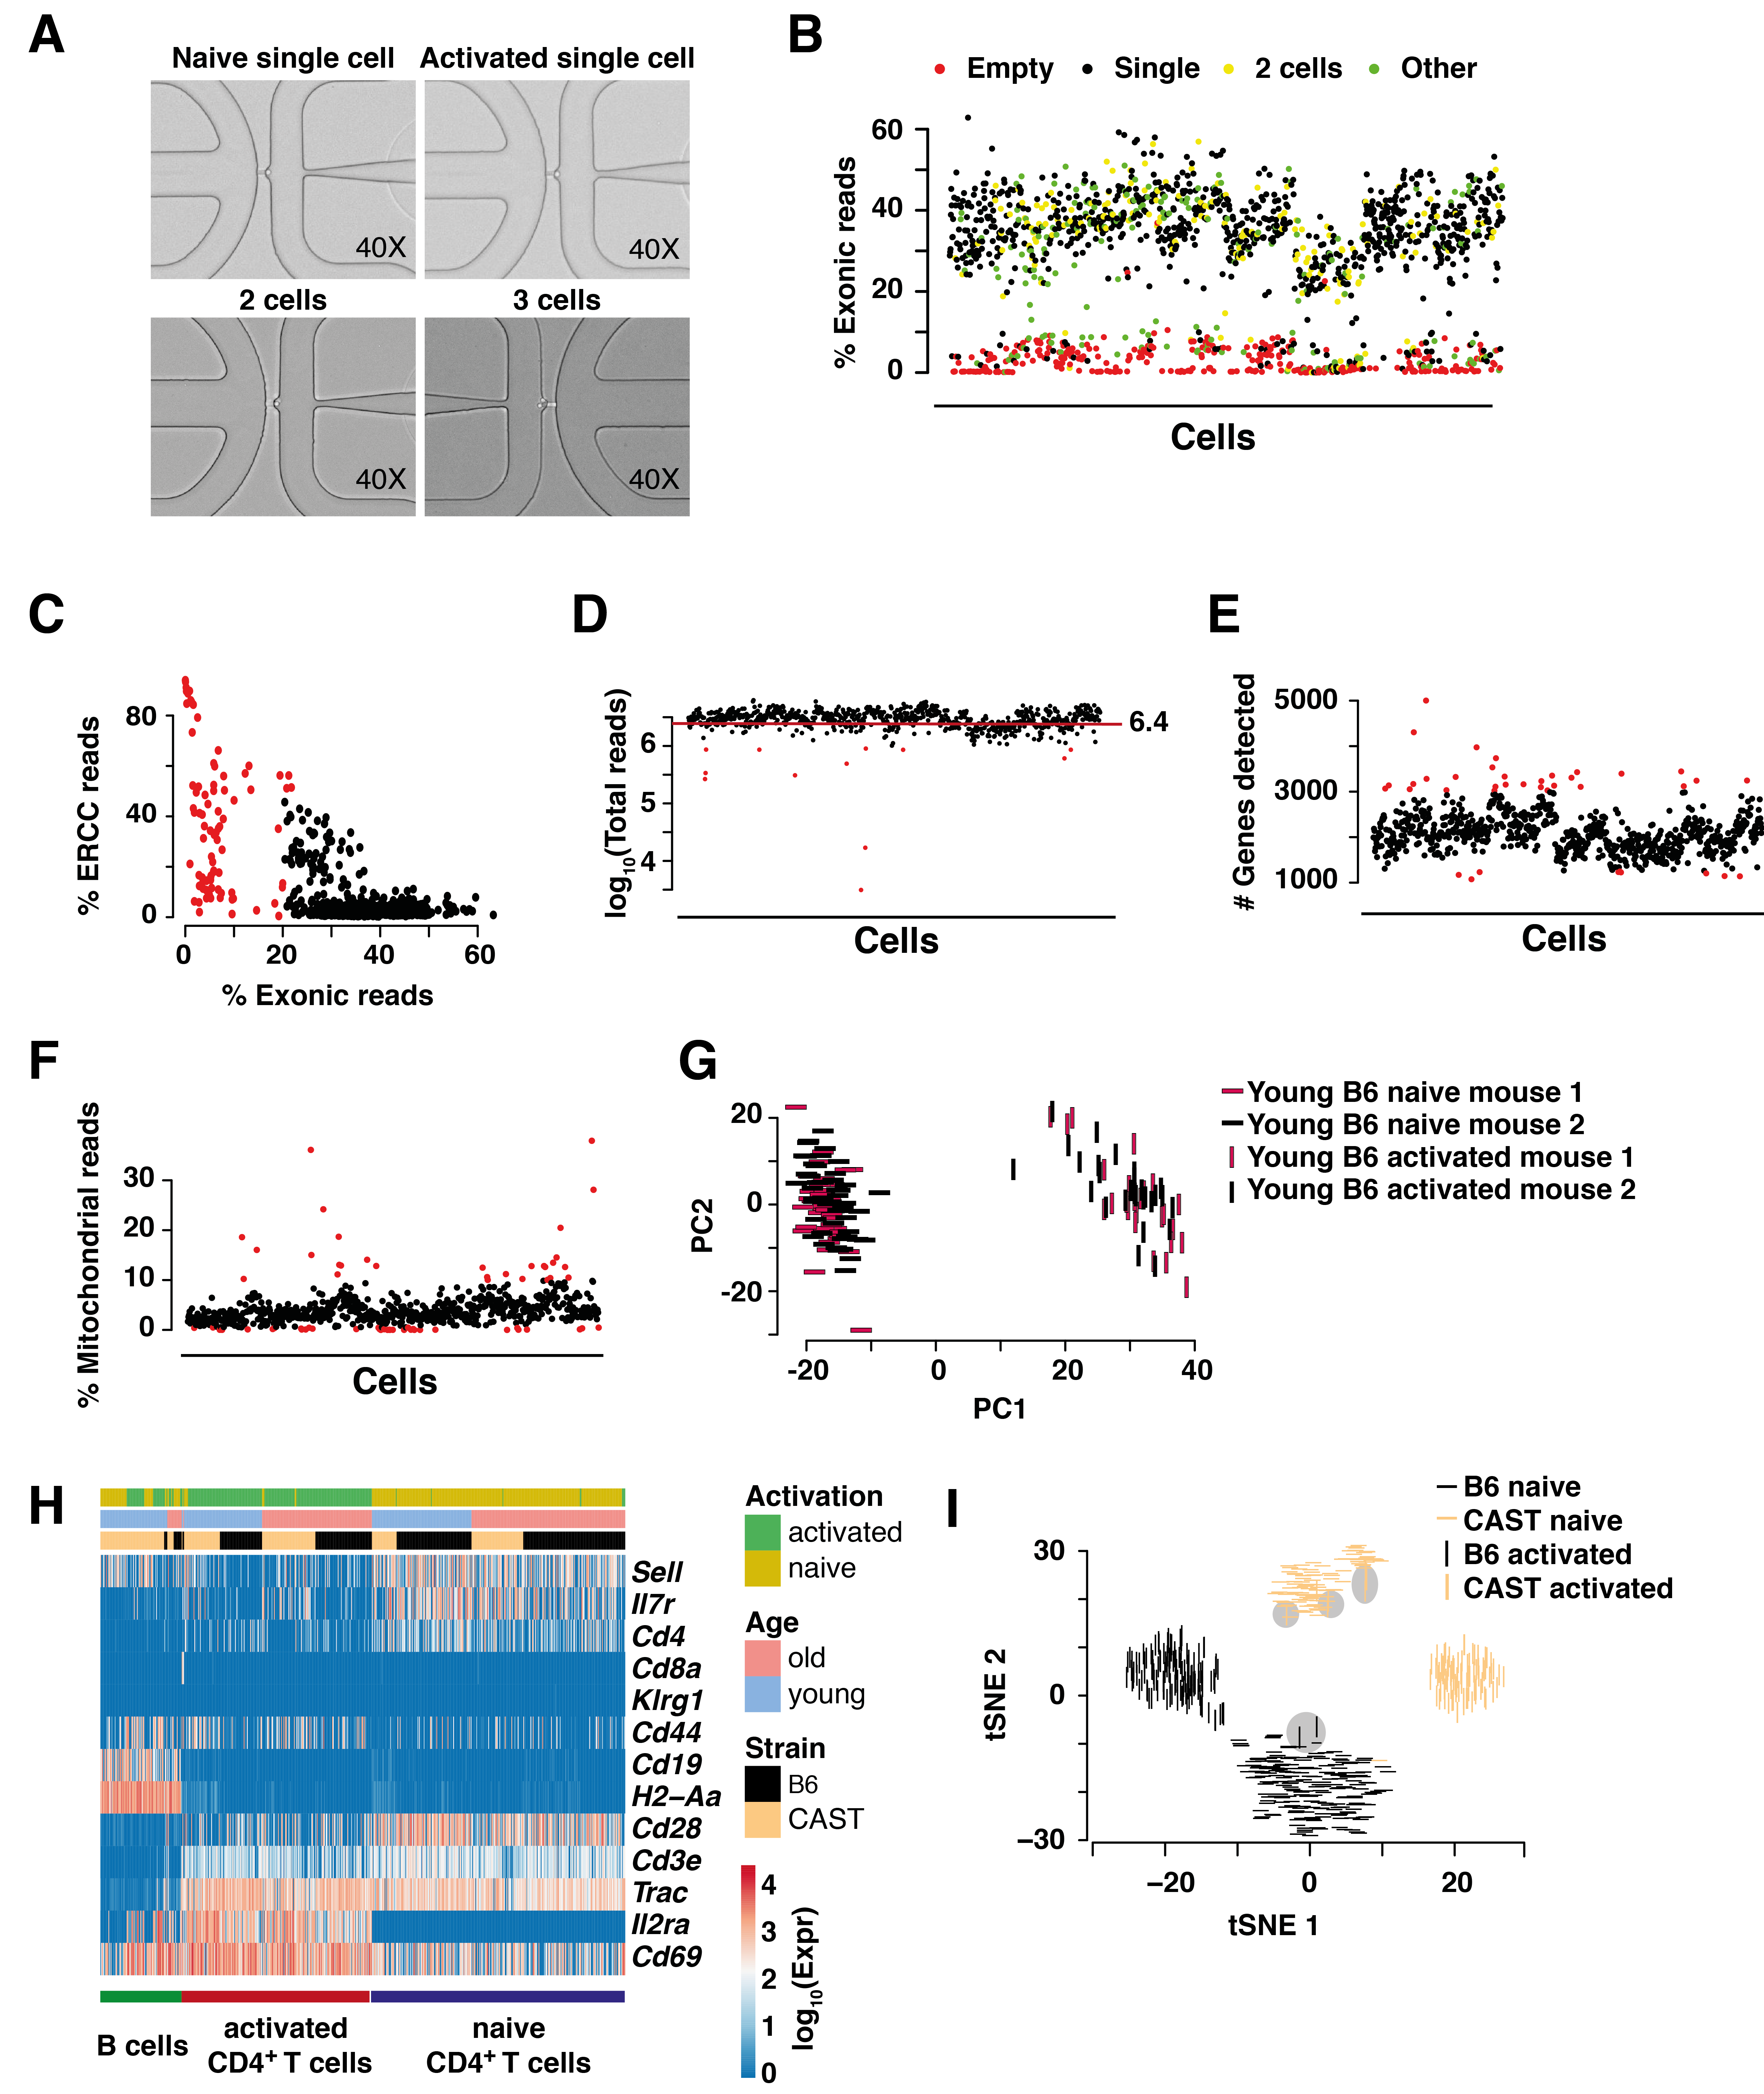
\includegraphics[width=0.9\textwidth,trim={0 4cm 0 0},clip]{Fig_3.png}
\caption[Quality control of isolated CD4$^+$ T cells]{\textbf{Quality control of isolated CD4$^+$ T cells (Full legend on next page).}}
\label{fig1:QC}
\end{figure}

\newpage

\captionsetup[figure]{list=no}
\addtocounter{figure}{-1}   
\captionof{figure}{\textbf{Quality control of isolated CD4$^+$ T cells (continued).}\\
\textbf{(A)} Visual inspection of captured cells at 40x magnification in Integrated Fluidic Circuit (C1, Fluidigm) allows manual removal of empty capture sites, and capture sites holding multiple cells or debris \textbf{(B)} Percentage of reads mapping to exonic regions displayed for naive and activated CD4$^+$ T cells. Black dots: single cells; yellow dots: 2 cells, red dots: empty wells, green dots: debris, multiple cells, etc.; \textbf{(C)} Removal of cells with less than 20\% of mapped exonic reads and more than 50\% of ERCC spike-in reads (red dots);
\textbf{(D)} Cells with less than 1 million mapped reads were excluded from downstream analysis (red dots);  \textbf{(E)} Cells with more than 3000 or less than 1250 genes detected were excluded in the analysis (red dots); \textbf{(F)} Cells with more than 10\% or less than 0.5\% of mitochondrial reads were excluded for downstream analysis (red dots); \textbf{(G)} Naive and activated cells isolated from young B6 animals (replicates) were coloured batch-specifically. 4 batches from 2 mice: naive and activated from mouse 1 (white bars), naive and activated from mouse 2 (black bars). Naive condition is represented in horizontal bars and activated condition in vertical bars; \textbf{(H)} Data set was filtered for immune markers to exclude B cell and CD8$^+$ T cell contamination. Cells in columns were labelled based on their activation state (naive in beige, activated in green), their age (old in red, young in blue), and the strain of the animals (B6 in black, CAST in yellow); \textbf{(I)} Unbiased tSNE clustering allowed the removal of not fully activated cells (indicated in grey circles). Cells were labelled based on their activation state (naive: horizontal bar, activated: vertical bar) and the strain of the animals (B6 in black, CAST in yellow).
.}
\captionsetup[figure]{list=yes}

\subsubsection*{Characterization of isolated CD4$^+$ T cells}

We determind the cell cycle stage of each cell using cyclone \citep{Scialdone2015} implemented in scran \citep{Lun2016}.
In contrast to haematopoeitic cells \citep{Kowalczyk2015}, even when activated, virtually all CD4$^+$ T cells are in G1 phase of cell cycle as expected \textbf{(Fig. \ref{fig1:characterization}A)}. Aged CD4$^+$ T cells showed no clonal expansions \textbf{(Fig. \ref{fig1:characterization}B)} or difference in cell size \textbf{(Fig. \ref{fig1:characterization}C)} that could impact analysis of gene expression variability \citep{Stubbington2015}. Using flow cytometry analysis, we confirmed that 96.4\% of the isolated CD4+ T cells were naive in young B6 \textbf{(Fig. \ref{fig1:characterization}D)}. Naive CD4+ T cells formed a single, high-purity population in young animals. Old animals had a small population of CD4$^+$ T cells with slightly elevated CD44 levels, reduced CD62L expression, and attenuated activation dynamics \textbf{(Fig. \ref{fig1:characterization}E-G)}. Upon T cell receptor (TCR) activation in the presence of particular cytokines, naive CD4$^+$ T cells can differentiate into several lineages of functionally different T helper cells (mainly Th1, Th2, Th17, Treg, Tfh) \citep{Stubbington2015, Zhu2010}. In our data we do not detect any early differentiation in naive and activated CD4$^+$ T cell subsets. In accordance with the literature we found \textit{Gata3} but not Th2 cytokines expressed in the majority of cells  \citep{Ho2009}. Interestingly, the Th1-related genes \textit{Tbx21} and \textit{Ifng} were up-regulated, in an uncoordinated manner, in a small population of activated CD4$^+$ T cells of old animals. This is consistent with a known Th1 bias in CD4$^+$ T cell responses in old mice \citep{Zhang2014} and humans \citep{Sakata-Kaneko2000} \textbf{(Fig. \ref{fig1:characterization}H)}. Furthermore, we did not detect any difference in TCR components/signaling and importantly detected no signs of T cell exhaustion \citep{Wherry2011}, especially in cells isolated from old animals \textbf{(Fig. \ref{fig1:characterization}I)}. We also ruled out species-specific differences in commitment towards T helper cell lineages \textbf{(Fig. \ref{fig1:characterization}J-K)}. \\

\begin{figure}[!hb]
\centering
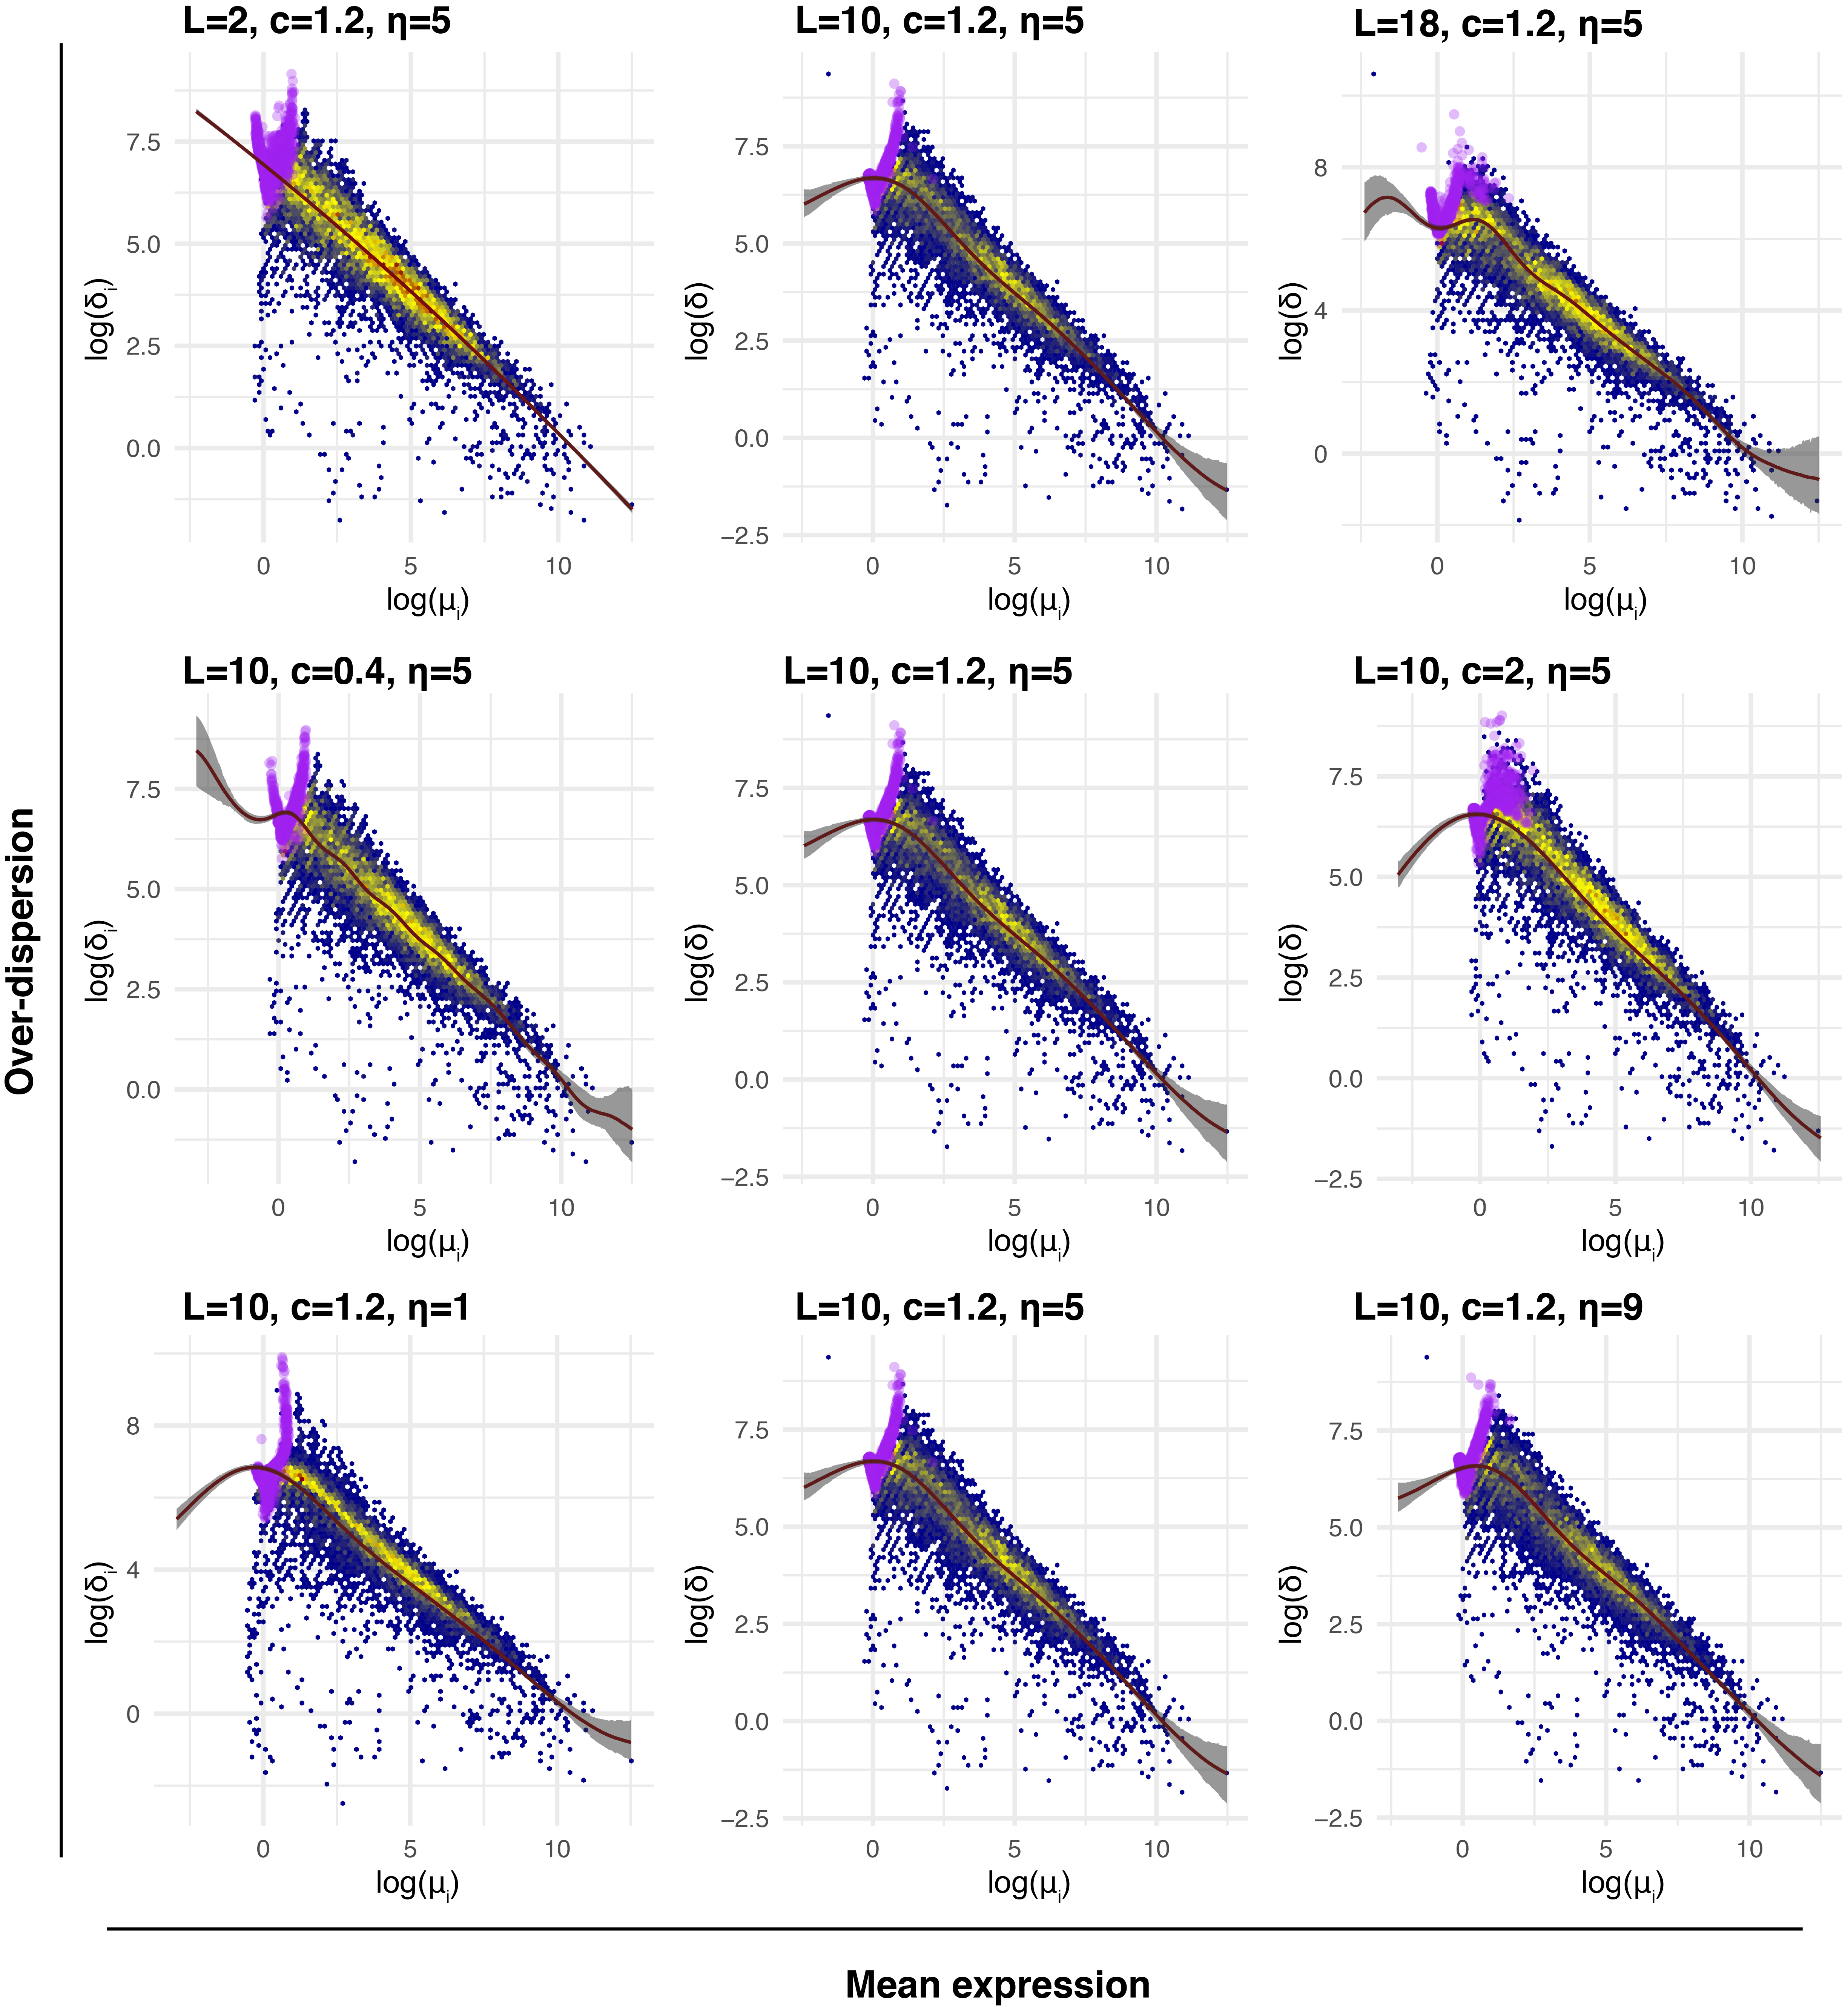
\includegraphics[width=0.8\textwidth]{Fig_4.png}
\caption[Characterization of isolated CD4$^+$ T cells]{\textbf{Characterization of isolated CD4$^+$ T cells (Full legend on next page).}}
\label{fig1:characterization}
\end{figure}

\newpage
\captionsetup[figure]{list=no}
\addtocounter{figure}{-1}   
\captionof{figure}{\textbf{Characterization of isolated CD4$^+$ T cells (continued).}\\
\textbf{(A)} Cyclone \citep{Scialdone2015} was used to classify individual naive and activated CD4+ T cells into the cell cycle phases G1, G2/M and S; \textbf{(B)} TraCeR \citep{Stubbington2015} constructed T cell receptor sequences from scRNA-seq data to analyze clonal diversity in naive and activated CD4$^+$ T cells; \textbf{(C)} Cell sizes were estimated for naive and activated CD4$^+$ T cells in young and old B6 animals measured by forward scatter (FSC-A) using flow cytometry; \textbf{(D)-(E)} CD4$^+$ T cells were purified from spleens of young (D) and old (E) B6 animals and stained with antibodies against CD4, CD62L, CD44, CD69, IL2R$\alpha$ (CD25), CD127, and KLRG1 as well as viability dye. FACS plots shown are gated on single live cells (top left panel) and single live CD4$^+$ T cells (other panels), and percentages shown relate to total of gated cells; \textbf{(F)-(G)} Naive CD4$^+$ T cells were purified from spleens of five young (F) or two aged (G) B6 mice, and were left naive or were activated with plate-bound antibody against CD3$\epsilon$ and CD28 for 3 hours. Cells were stained with antibodies against CD4, CD69, and viability dye. Representative histograms are shown and were gated on single live CD4$^+$ T cells: naive (red) and activated (blue) cells are shown; \textbf{(H)} Characterization of possible differentiation processes leading to T helper 1 (Th1), T helper 2 (Th2), T helper 17 (Th17), regulatory T (Treg) and follicular helper T (Tfh) cell lineages. For each lineage the major regulatory transcription factor (upper row) and an effector cytokine (lower row) is shown. Statistical differential expression testing was performed between activated and naive cells from young B6 animals (left panel) and between activated and naive cells from old B6 animals (right panel). Upward arrow: up-regulation of expression (log2FC > 2, FDR < 0.05) after activation, Downward arrow: down-regulation of expression (log2FC > 2, FDR < 0.05) after activation; \textbf{(I)} Heatmap showing T cell exhaustion (Pdcd1, Lag3, Havcr2, Ctla4) and TCR activation markers (Cd5). Statistical differential expression testing was performed in naive cells between young and old B6 animals (left panel) and in activated cells between young and old B6 animals (right panel). Upward arrow: up-regulation of expression (log2FC > 2, FDR < 0.05) during aging; \textbf{(J)} Th1 lineage marker (Tbx21, Ifng) expression was compared between B6 and CAST in following conditions: naive cells from young animals (upper left panel), naive cells from old animals (lower left panel), activated cells from young animals (upper right panel), activated cells from old animals (lower right panel). \#: statistically significant differential expression (log2FC > 2, FDR < 0.05); \textbf{(K)} Th2 lineage marker (Gata3, Il4) expression was compared between B6 and CAST in following conditions: naive cells from young animals (upper left panel), naive cells from old animals (lower left panel), activated cells from young animals (upper right panel), activated cells from old animals (lower right panel).
\\}
\captionsetup[figure]{list=yes}

After the above analyses and the experimental characterization, a total of 1514 high-quality CD4$^+$ T cell transcriptomes were analysed across all conditions and species. An overview of all high-quality transcriptomes can be seen in \textbf{Fig. \ref{fig1:all_cells}}. We detect that unstimulated and stimulated cells group together \textbf{(Fig. \ref{fig1:all_cells}A)} while separation is also noticeable between strains \textbf{(Fig. \ref{fig1:all_cells}B)} and experimental methods \textbf{(Fig. \ref{fig1:all_cells}C)}. As discussed below, cells from young and old animals do not separate when visualizing the cells in form of a t-distributed stochastic neighbour embedding (tSNE, \textbf{Fig. \ref{fig1:all_cells}C}). 

\newpage

\begin{figure}[!hb]
\centering
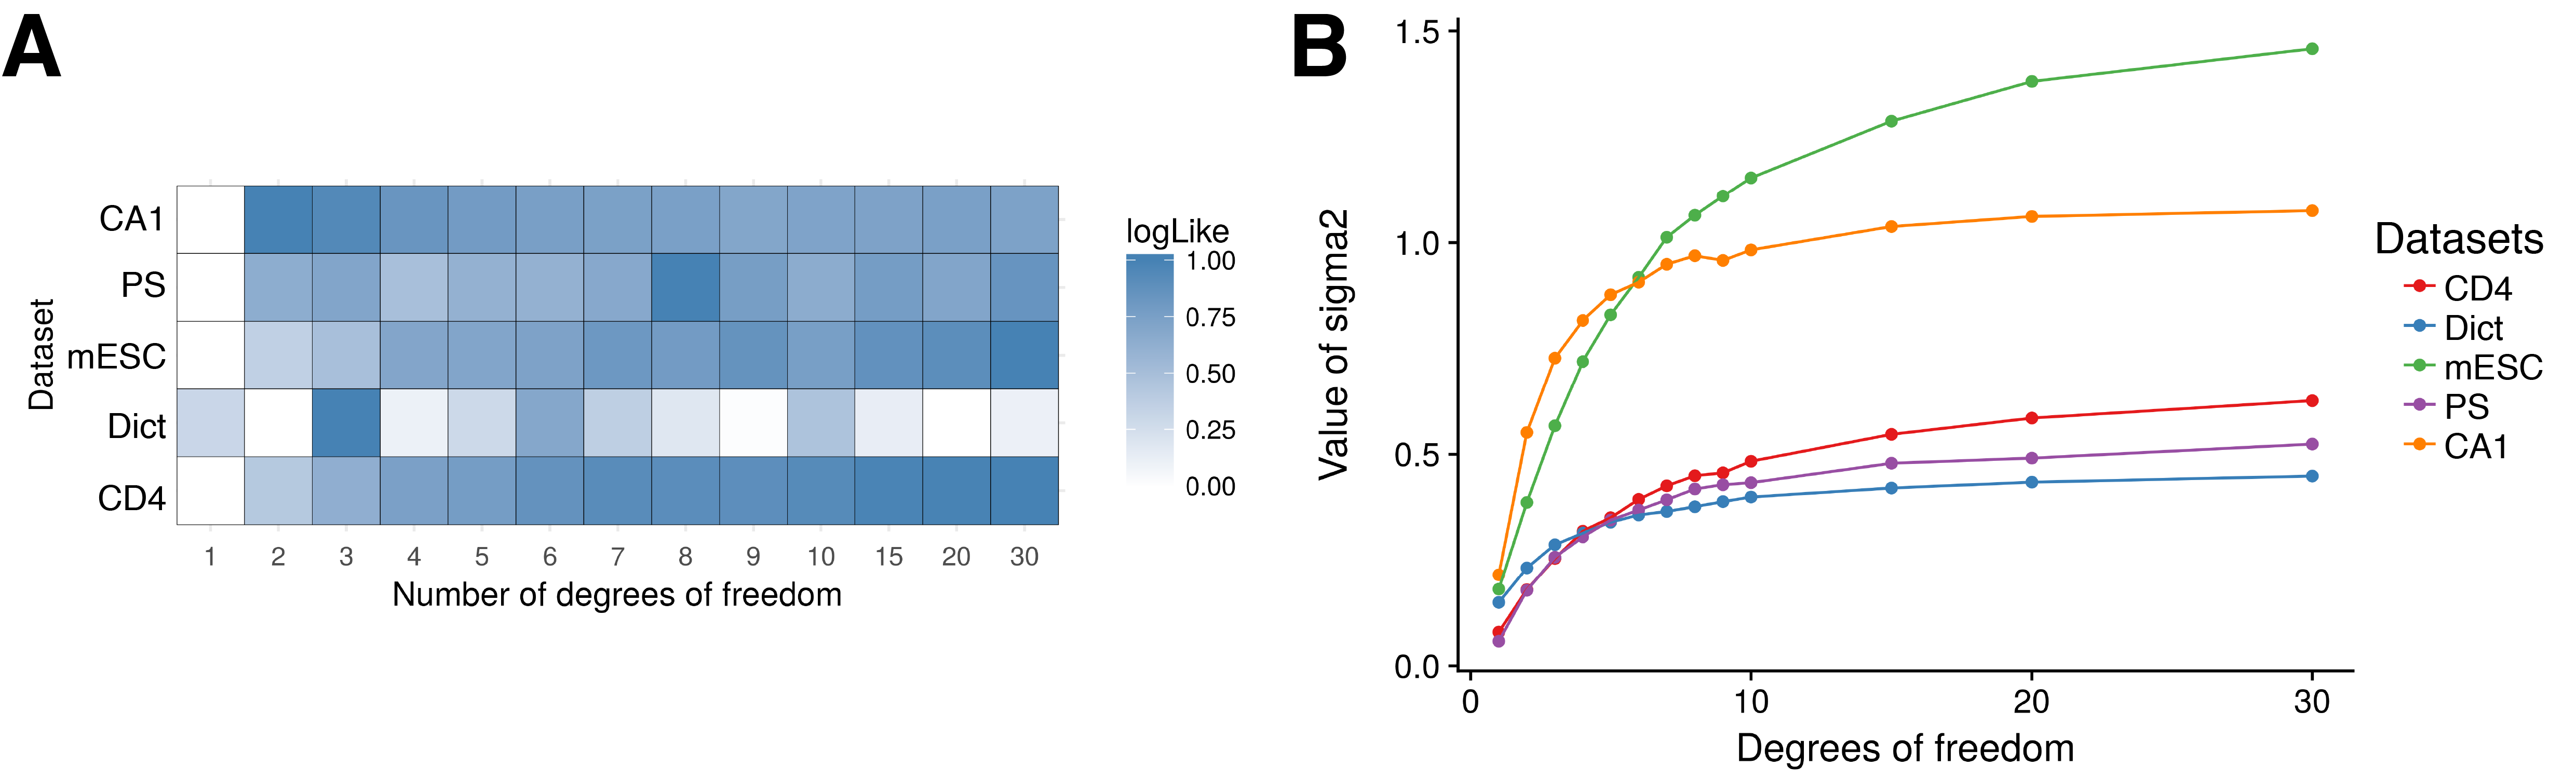
\includegraphics[width=0.8\textwidth]{Fig_5.png}
\caption[Visualization of all isolated CD4$^+$ T cells]{\textbf{Visualization of all isolated CD4$^+$ T cells.}\\
tSNE dimensionality reduction of 1514 CD4$^+$ T cells isolated from young and old mice of two related strains. Cells were labelled based on \textbf{(A)} their activation state, \textbf{(B)} the mouse strain, \textbf{(C)} experimental isolation approach and \textbf{(D)} age.}
\label{fig1:all_cells}
\end{figure}

\begin{Comment}
\textbf{Box 2: BASiCS parameter estimation using transcriptomes of CD4$^+$ T cells}\\
To quantify and assess changes in mean expression and expression variability, we used the Bayesian hierarchical framework BASiCS introduced in section \ref{sec0:BASiCS}. The Markov Chain Monte-Carlo (MCMC) simulation was run on quality filtered transcriptomes of CD4$^+$ T cells condition-specifically. We used posterior medians of $\mu_i$ to capture mean expression and posterior medians of the over-dispersion parameter $\delta_i$ to quantify biological expression variability. Differential mean expression testing was performed using a probabilistic decision rule of $\log_2(\mu_i^{(A)}/\mu_i^{(B)})>\tau_0$ being larger than a given probability threshold (\emph{e.g.} 80\%). Here, A and B indicate the different conditions and $\tau_0$ is the chosen minimum tolerance threshold. The decision rule associated to differential variability testing is: $\log_2(\delta_i^{(A)}/\delta_i^{(B)})>\omega_0$. Due to the strong confounding between mean expression $\mu_i$ and over-dispersion $\delta_i$ (as described in section \ref{sec0:BASiCS}), we only consider genes with no changes in mean expression ($\tau_0=0$, FDR<0.05) to assess changes in variability. Throughout this chapter, the decision rule is abbreviated with: log2FC. 
\end{Comment}

\newpage

\section{Species-specific gene expression in naive CD4$^+$ T cells}
\subsection*{Single-cell RNA-seq reveals species-specific gene expression in naive CD4$^+$ T cells}

To fully characterize the variation observed in \textbf{Fig. \ref{fig1:all_cells}}, we dissected differences in gene expression between the two different mouse strains for naive CD4$^+$ T cells. Similar for \textbf{Fig. \ref{fig1:all_cells}}, we found that naive CD4+ T cells cluster by species when only profiling naive CD4$^+$ T cells \textbf{(Fig. \ref{fig1:species_specific})}.

\begin{figure}[!h]
\centering
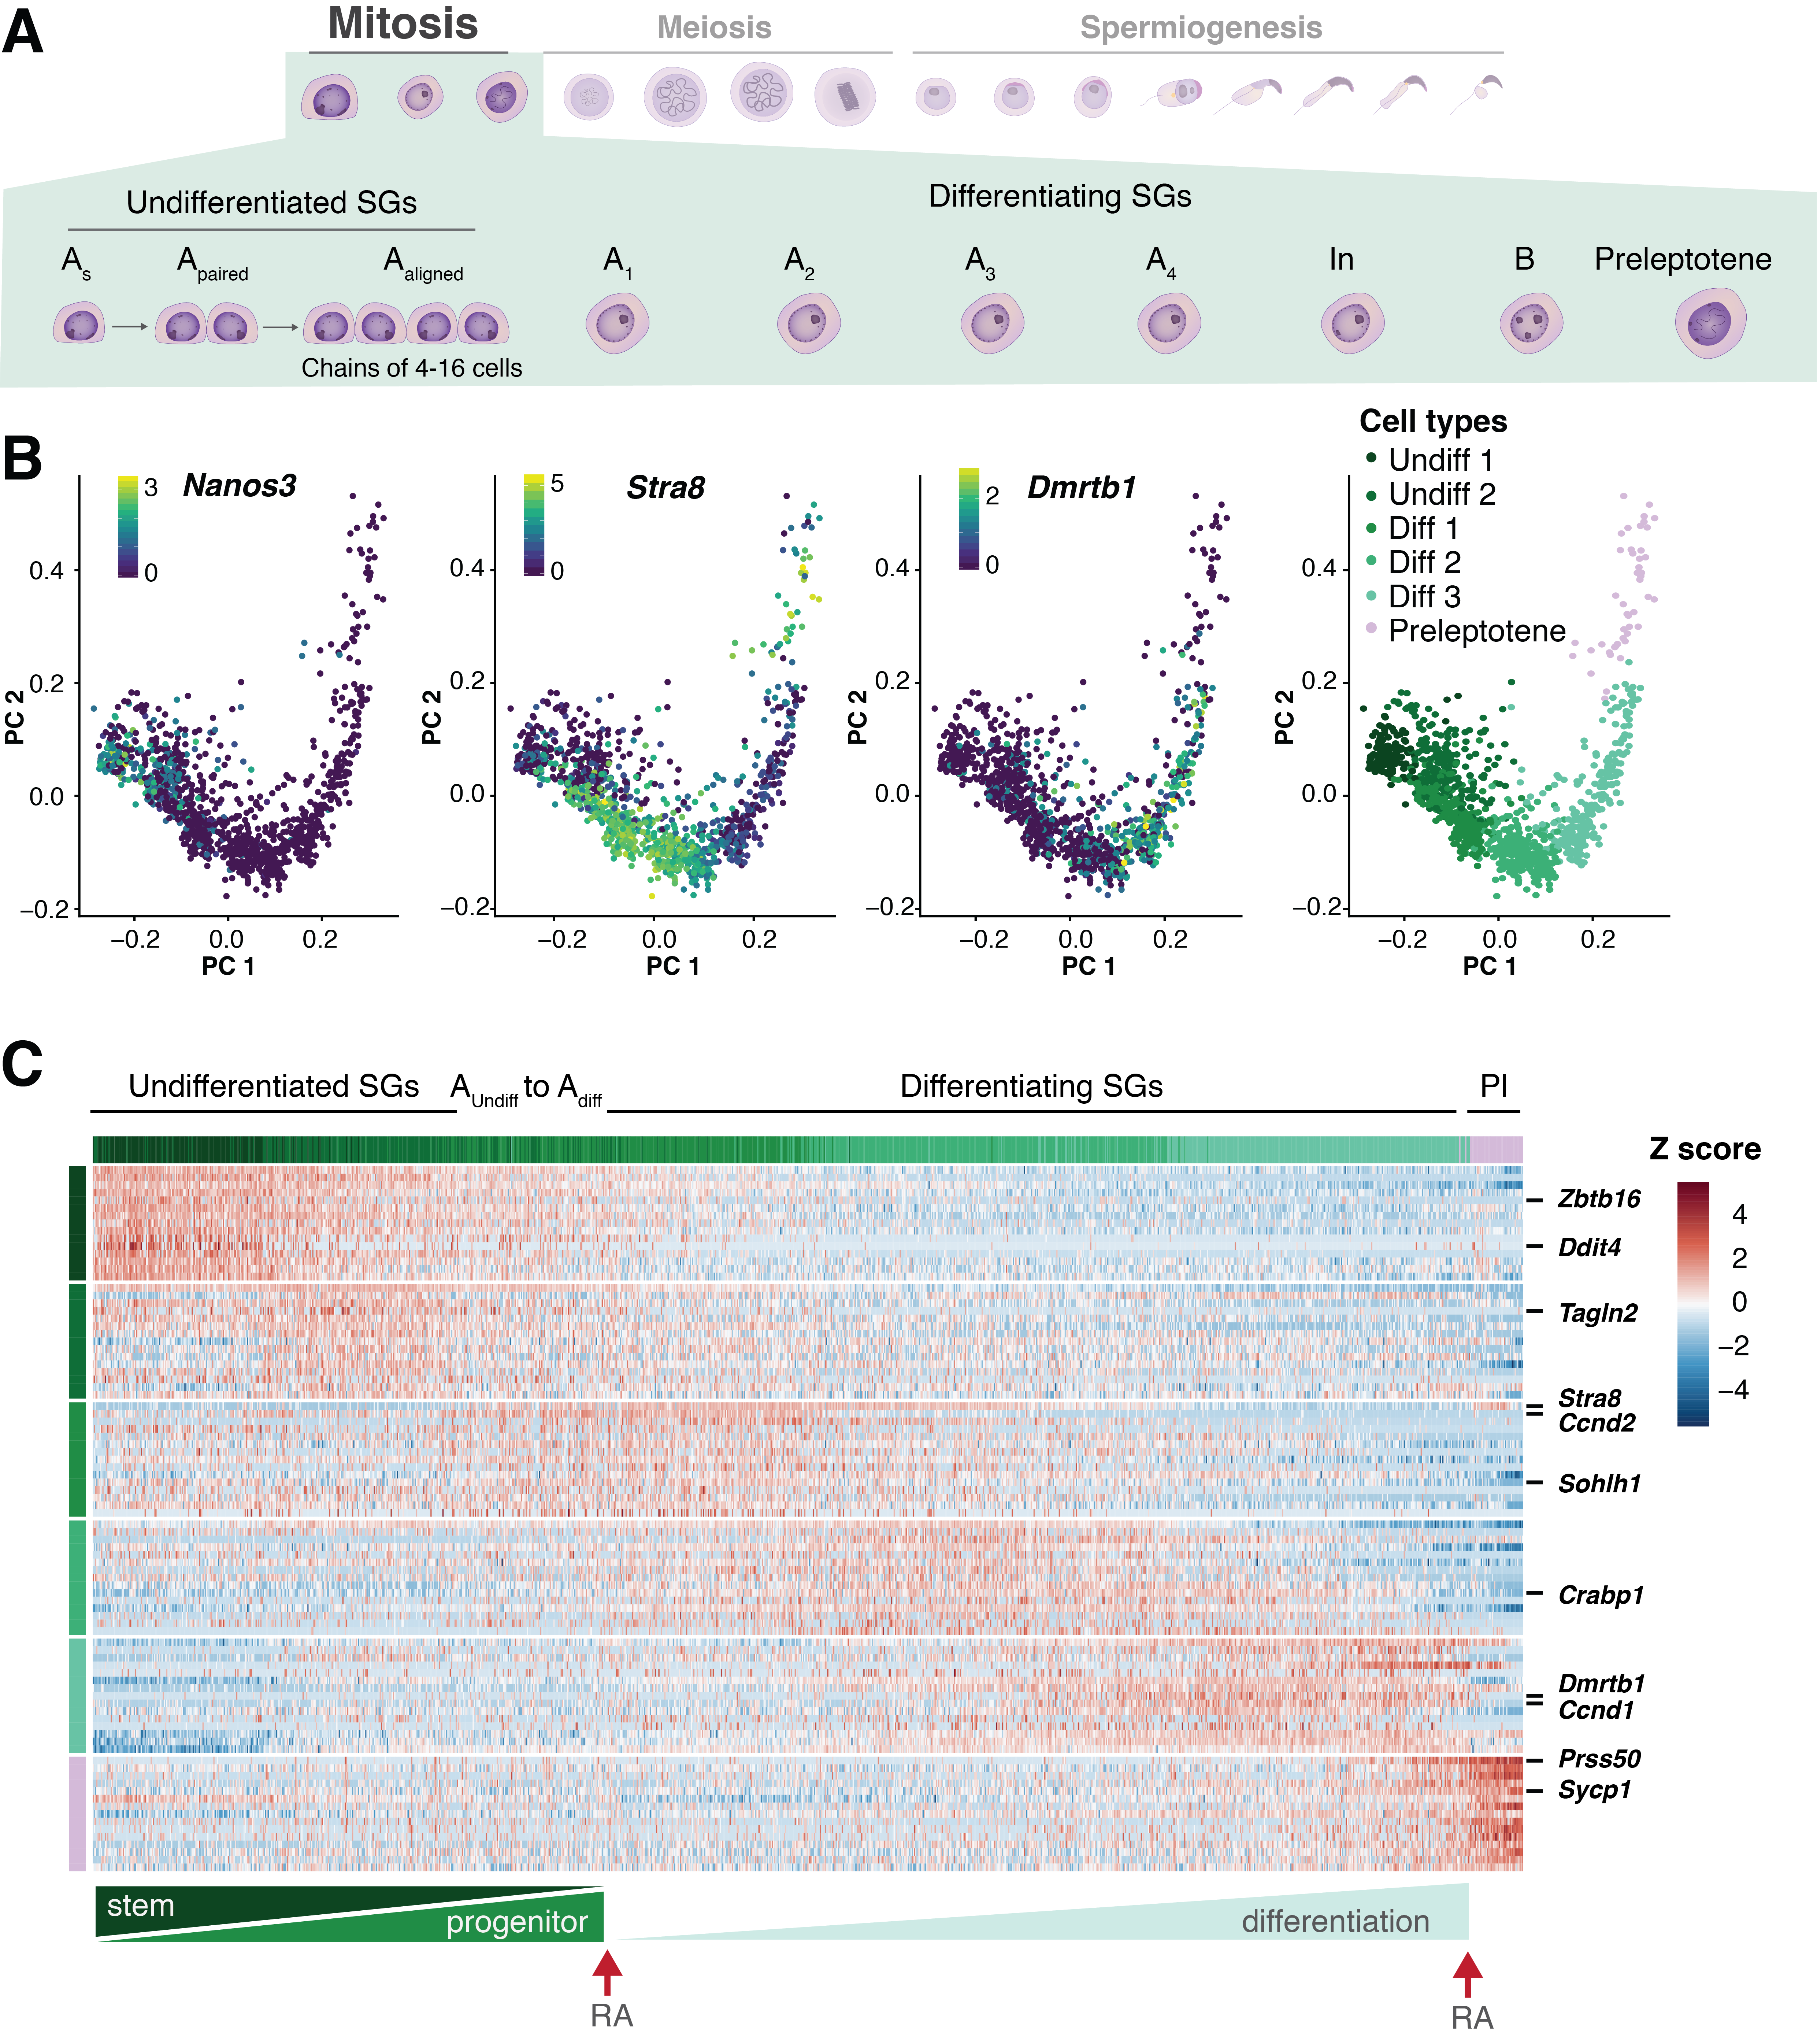
\includegraphics[width=0.9\textwidth]{Fig_6.png}
\caption[Species-specific gene expression in naive CD4$^+$ T cells]{\textbf{Species-specific gene expression in naive CD4$^+$ T cells.}\\
\textbf{(A)} tSNE dimensionality reduction of scRNA-seq data reveals species-specific clustering of naive CD4$^+$ T cells from young animals; \textbf{(B)} Representative heatmap of 30 genes and 30 cells randomly selected from all species-specifically transcribed genes from young animals shows typical species-specific variation; \textbf{(C)}  GO analysis of species-specific genes. Bonferroni corrected p-values (adjusted p-values) were used to visualize GO enrichment. The statistical significance threshold was set to adjusted p-value < 0.1 (red line); \textbf{(D)} Cell-to-cell variability in gene expression levels; violin plots show distribution of single-cell expression of selected species-specifically transcribed genes (in grey background), ranked from lowest (top) to highest variability (bottom); \textbf{(E)} $\log_10$-transformed variability estimates of species-specific genes were compared to variability estimates of all genes expressed in B6 (left) and CAST (right). Mann-Whitney-Wilcoxon test; ***: p<10-10}
\label{fig1:species_specific}
\end{figure}

\newpage

We used BASiCS to detect differentially expressed and differentially variable genes. For changes in mean expression between populations, we first excluded genes that had an average posterior mean expression rate < 50 in each population. Subsequently, we applied the differential expression test developed within BASiCS, using a threshold of log2FC > 2 with an FDR cutoff of 0.05 (see \textbf{Box 2}). We observed that 15\% of expressed genes were transcribed differentially between the two mouse species’ CD4$^+$ T cells \textbf{(Fig. \ref{fig1:spec_spec_mapping}A)}. To rule out the possibility that this clustering is driven by potential artefacts in the new \textit{Mus musculus castaneus} genome assembly, we also mapped reads from young CAST samples to the GRCm38 genome. To estimate which differentially expressed genes may arise due to errors in the new CAST genome assembly, we performed the same differential expression analysis on CAST samples by mapping these experiments onto both GRCm38 and CAST. Roughly 5\% of all tested genes are detected as differentially expressed even though the samples being compared are identical and only mapped to different genomes \textbf{(Fig. \ref{fig1:spec_spec_mapping}B)}. Comparing this set of genes to the set of species-specific genes, we find that they make up 10\% of differentially expressed genes between the two species. We performed a similar analysis for B6 samples. This approach allowed us to remove from our analyses the genes showing differences in expression, which may be driven by the quality of the reference genome. These genes were removed from further analyses.

\begin{figure}[!hb]
\centering
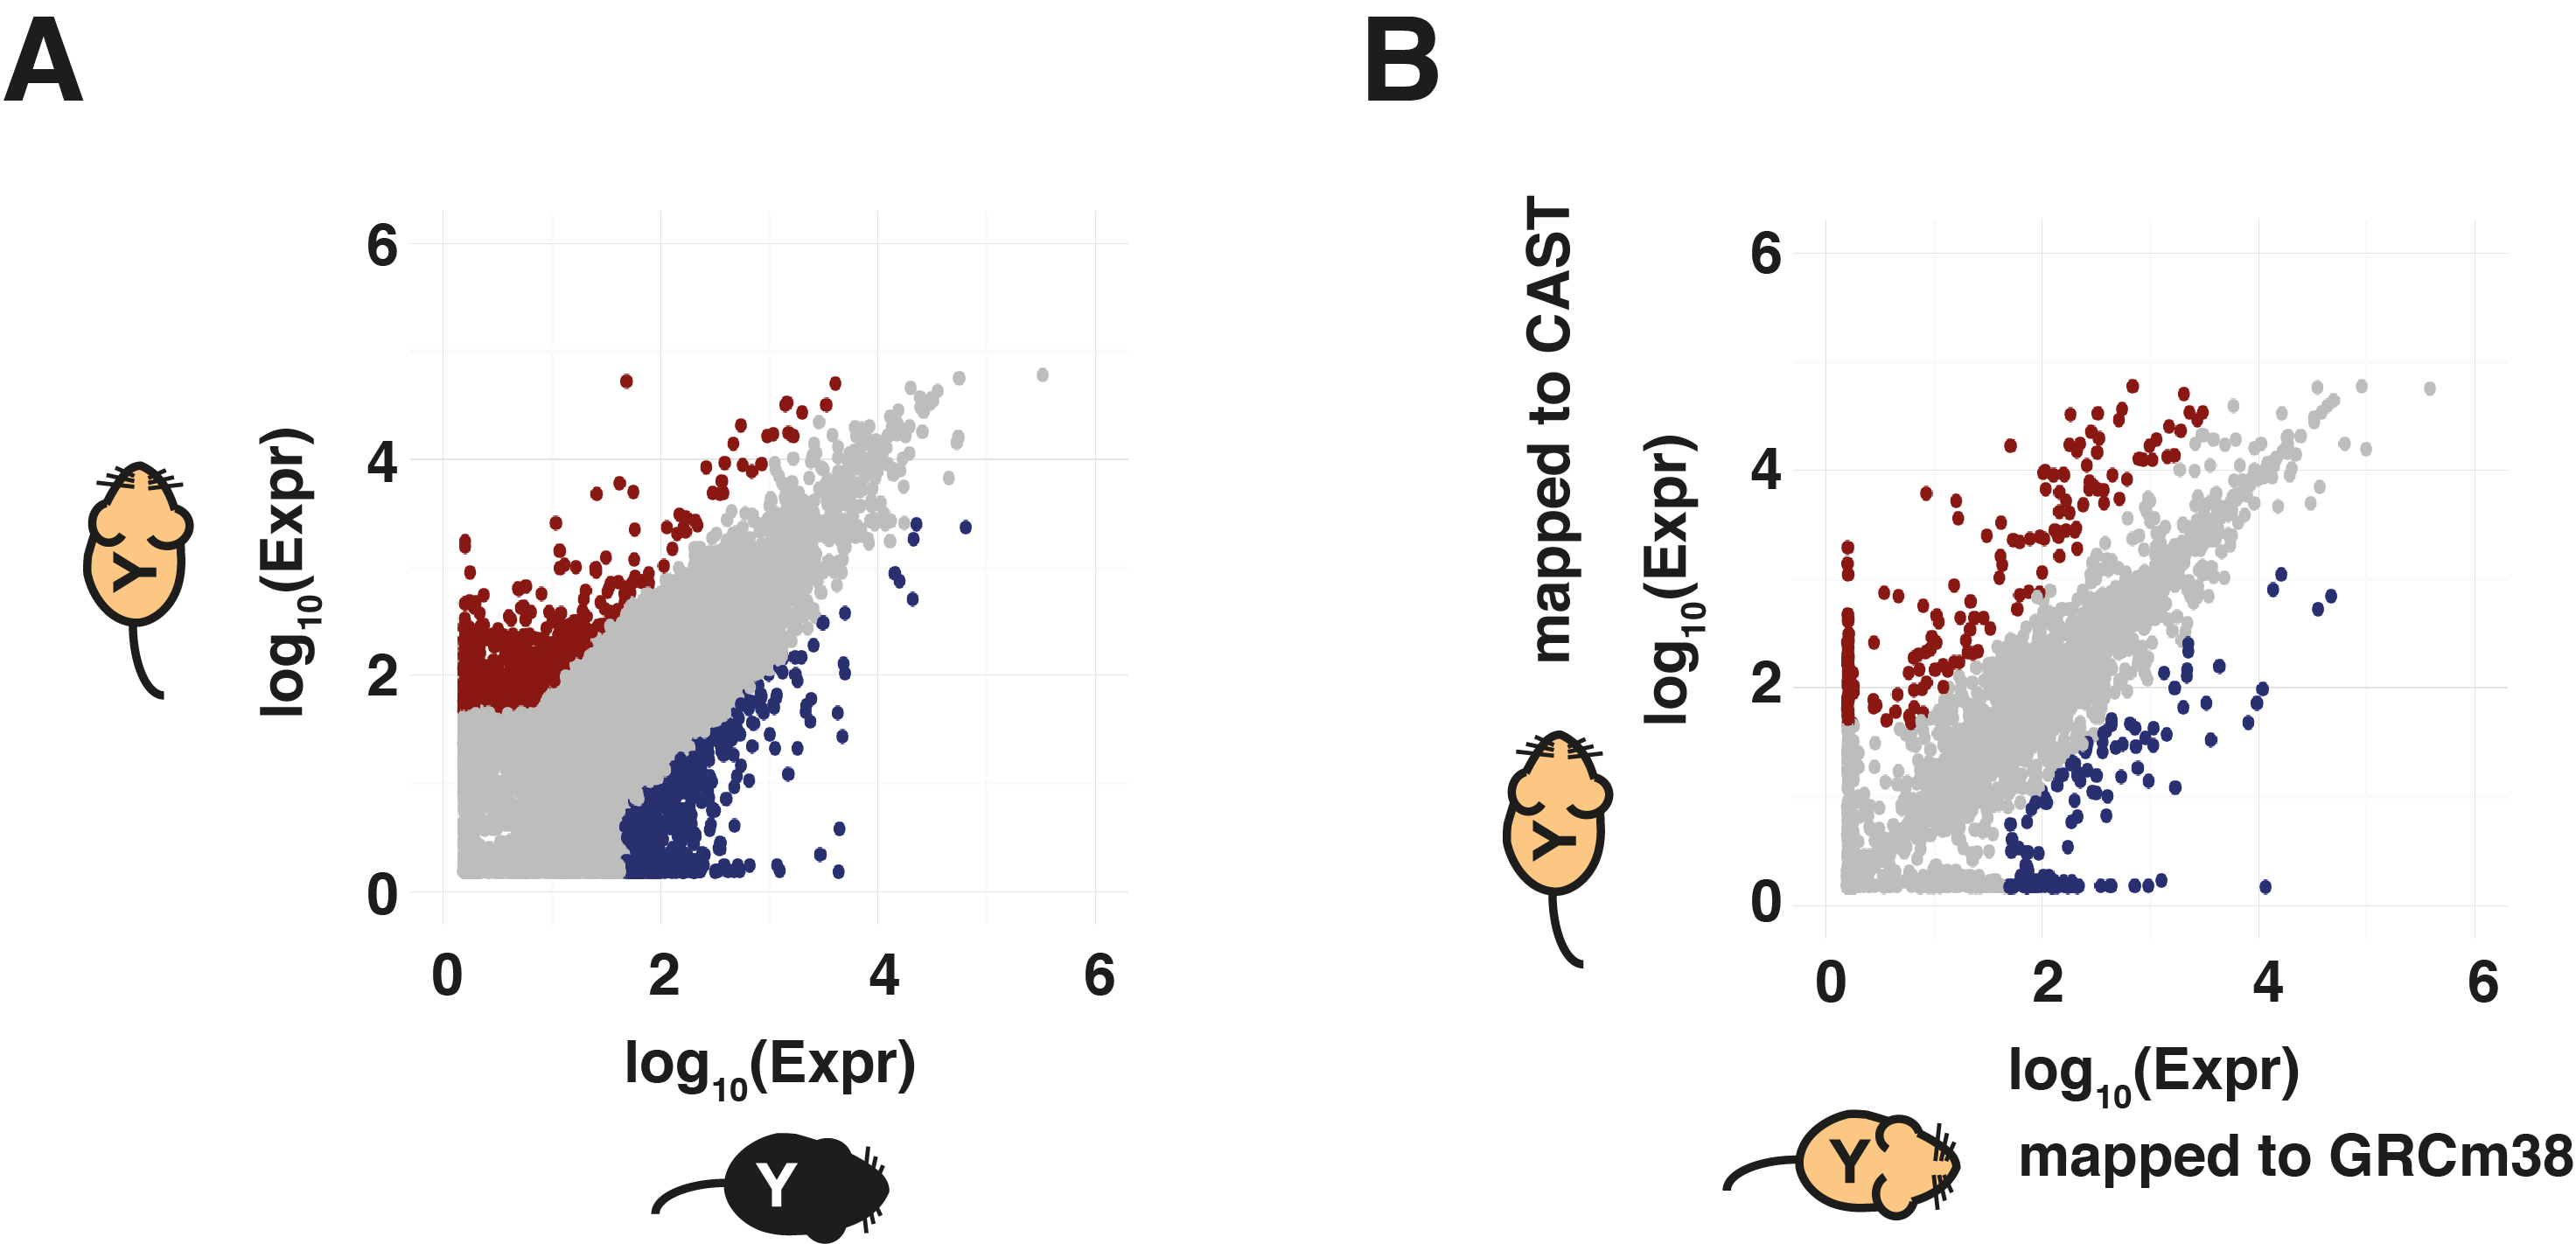
\includegraphics[width=0.8\textwidth]{Fig_7.png}
\caption[Cross-mapping correction between divergent mouse strains]{\textbf{Cross-mapping correction between divergent mouse strains.}\\
\textbf{(A)} Species-specific gene expression in B6 (blue) or CAST (red). Average gene expression using posterior estimation, threshold of means > 50, log2FC > 2, FDR < 0.05; \textbf{(B)} Mean, normalized transcript counts of mapped reads from CAST cells (young, naive) using the GRCm38 genome (x-axis) or the CAST genome (y-axis) as reference. Differentially mapped genes were removed from downstream analysis. Average gene expression using posterior estimation, threshold of means > 50, log2FC > 2, FDR < 0.05.
}
\label{fig1:spec_spec_mapping}
\end{figure}

To asses the functional role of the remaining species-specific genes, we qualitatively and quantitatively compared their expression across individual cells in both species. Firstly, species-specific genes were only expressed in subsets of the full population of naive CD4$^+$ T cells \textbf{(Fig. \ref{fig1:species_specific}B)}. Furthermore, we used DAVID (30) to test for gene ontology (GO) enrichment in differentially expressed genes and did not detect functional enrichment in either B6 or CAST specific genes \textbf{(Fig. \ref{fig1:species_specific})}. Profiling individual cells allows us to detect different patterns of expression variability for species-specific genes \textbf{(Fig. \ref{fig1:species_specific})}. Profiling expression variability, we detect species-specifically transcribed genes to be generally more variable on a cell-to-cell basis than genes expressed in both species \textbf{(Fig. \ref{fig1:species_specific}E)}. These findings hint at the detected divergence in genes expression being cause by neutral drift without functional support of the species-specific genes.

\section{Expression dynamics during CD4$^+$ T cell activation}
\subsection*{Early CD4$^+$ T cell activation induces a transcriptional switch from stochastic to tightly regulated gene expression} \label{sec1:Tcell_activation}

Functional CD4$^+$ T cell transcriptional responses start with an early, targeted activation of translational machinery and cytokine networks, followed by large-scale transcriptional changes associated with lineage commitment \citep{Shay2013, Asmal2003}. To characterize the immediate early activation program, we stimulated naive CD4$^+$ T cells for three hours with plate-bound anti-CD3$\epsilon$/anti-CD28 antibodies, thus inducing a strong and uniform activation mimicking initial contact with an antigen-presenting cell inducing strong transcriptional changes \textbf{(Fig. \ref{fig1:immune_activation})}. Importantly, we did not use additional cytokines to commit the naive CD4+ cells to specific helper cell lineages \citep{Zhu2010}. \\
Differential mean expression testing identifies thousands of genes being differentially expressed in CD4$^+$ T cells upon activation (2063 genes, log2FC>2) \textbf{(Fig. \ref{fig1:immune_activation}B)}. We sought to investigate the behaviour of up- and down-regulated genes across the population of naive or activated cells. Initially, we calculated, for each gene, the percentage of cells in which it was expressed (> 0 transcript counts). Genes whose expression is down-regulated after activation are expressed in 18\% of naive CD4+ T cells isolated from B6, while genes that are up-regulated are expressed in 36\% of activated cells (median fraction of cells in which gene expression was detected, 600 genes were randomly selected in each condition) \textbf{(Fig. \ref{fig1:immune_activation}C)}. Before activation, up-regulated genes are only expressed on average in 5\% of naive cells while after activation, down-regulated genes are expressed in 4\% of activated cells \textbf{(Fig. \ref{fig1:immune_activation}C)}. 

\newpage

\begin{figure}[!ht]
\centering
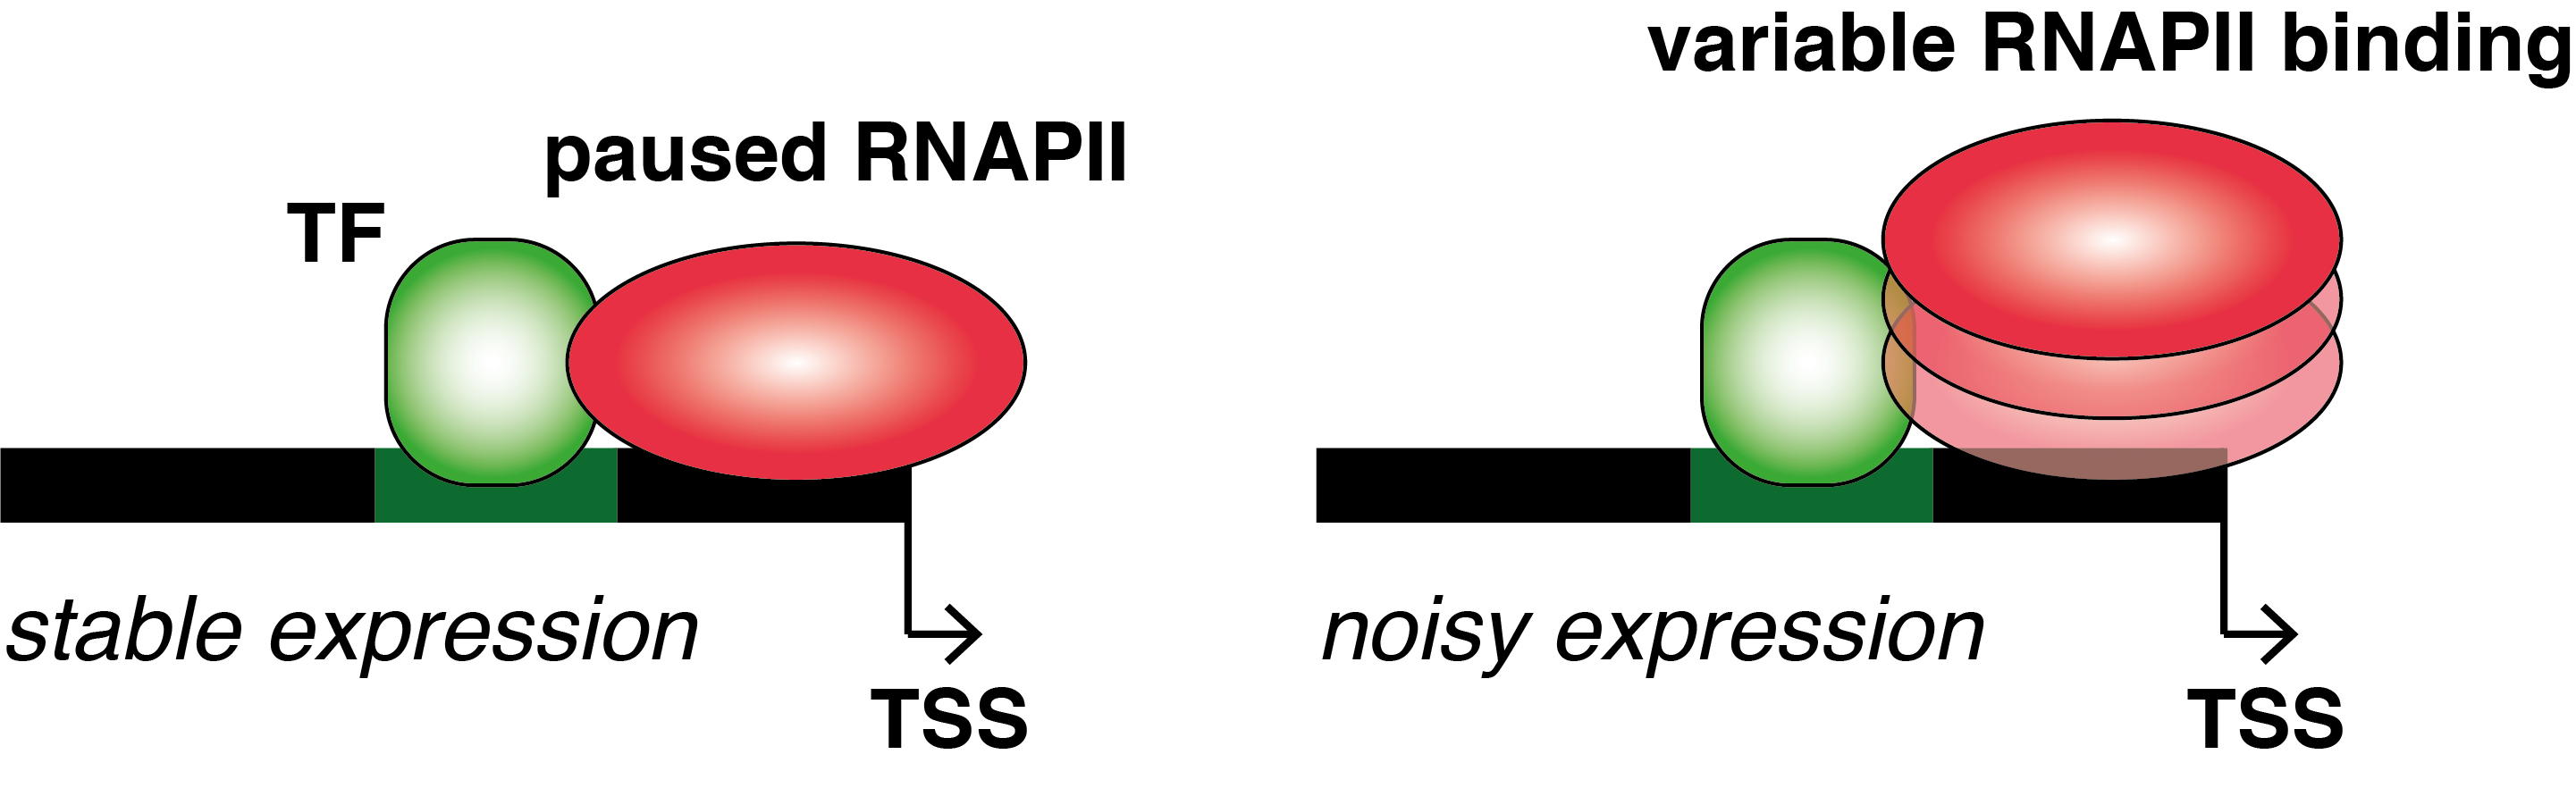
\includegraphics[width=0.9\textwidth]{Fig_8.png}
\caption[Mean expression dynamics upon CD4$^+$ T cell activation]{\textbf{Mean expression dynamics upon CD4$^+$ T cell activation.}\\
\textbf{(A)} Activation of CD4$^+$ T cells from young B6 mice induces large-scale transcriptional changes, visualized using tSNE dimensionality reduction; \textbf{(B)} Genes up-regulated (red) and down-regulated (blue) by immune stimulation in young B6 mice. Non-differentially expressed genes shown in black. Average gene expression using posterior estimation, threshold of means > 50, log2FC > 2, FDR < 0.05; \textbf{(C)} Fractions of cells in which down- or up-regulated genes are expressed (600 genes were randomly selected, histograms with 50 bins, median value is indicated). Upper panels: fraction of naive (left) and activated (right) cells in which down-regulated genes are expressed. Lower panels: fraction of naive (left) and activated (right) cells in which up-regulated genes are expressed; \textbf{(D)} Bar plots of functional gene categories enriched in up- and down-regulated genes during activation of CD4+ T cells in B6 (Bonferroni multiple testing corrected p-values, red line marking 0.1); \textbf{(E)} Example genes that represent transcriptional changes upon activation of CD4$^+$ T cells: \textit{Il2ra} (CD25) is highly and consistently up-regulated after stimulation; \textbf{(F)} \textbf{Cd62l} is stochastically expressed in naive CD4$^+$ T cells, and is down-regulated upon activation.
}
\label{fig1:immune_activation}
\end{figure}

Furthermore, we performed GO analysis on genes either up- or down-regulated \textbf{Fig. \ref{fig1:immune_activation}D}. Among the genes down-regulated are components of the intra-cellular signalling network while genes that are up-regulated are mostly part of the translation machinery \citep{Bjur2013}. Furthermore, the transcriptional switch driven by TCR engagement and co-stimulation included classic markers of activation, including interleukin 2 receptor alpha (\textit{Il2ra},\textbf{Fig. \ref{fig1:immune_activation}E}) and chemokine (c-c motif) ligand 4 (\textit{Ccl4}) \citep{Asmal2003}. In contrast, we observed the coordinated suppression of \textit{Sell} (\textit{Cd62l}, \textbf{Fig. \ref{fig1:immune_activation}F}), as expected after activation \todo{[REF]}.


\begin{figure}[!ht]
\centering
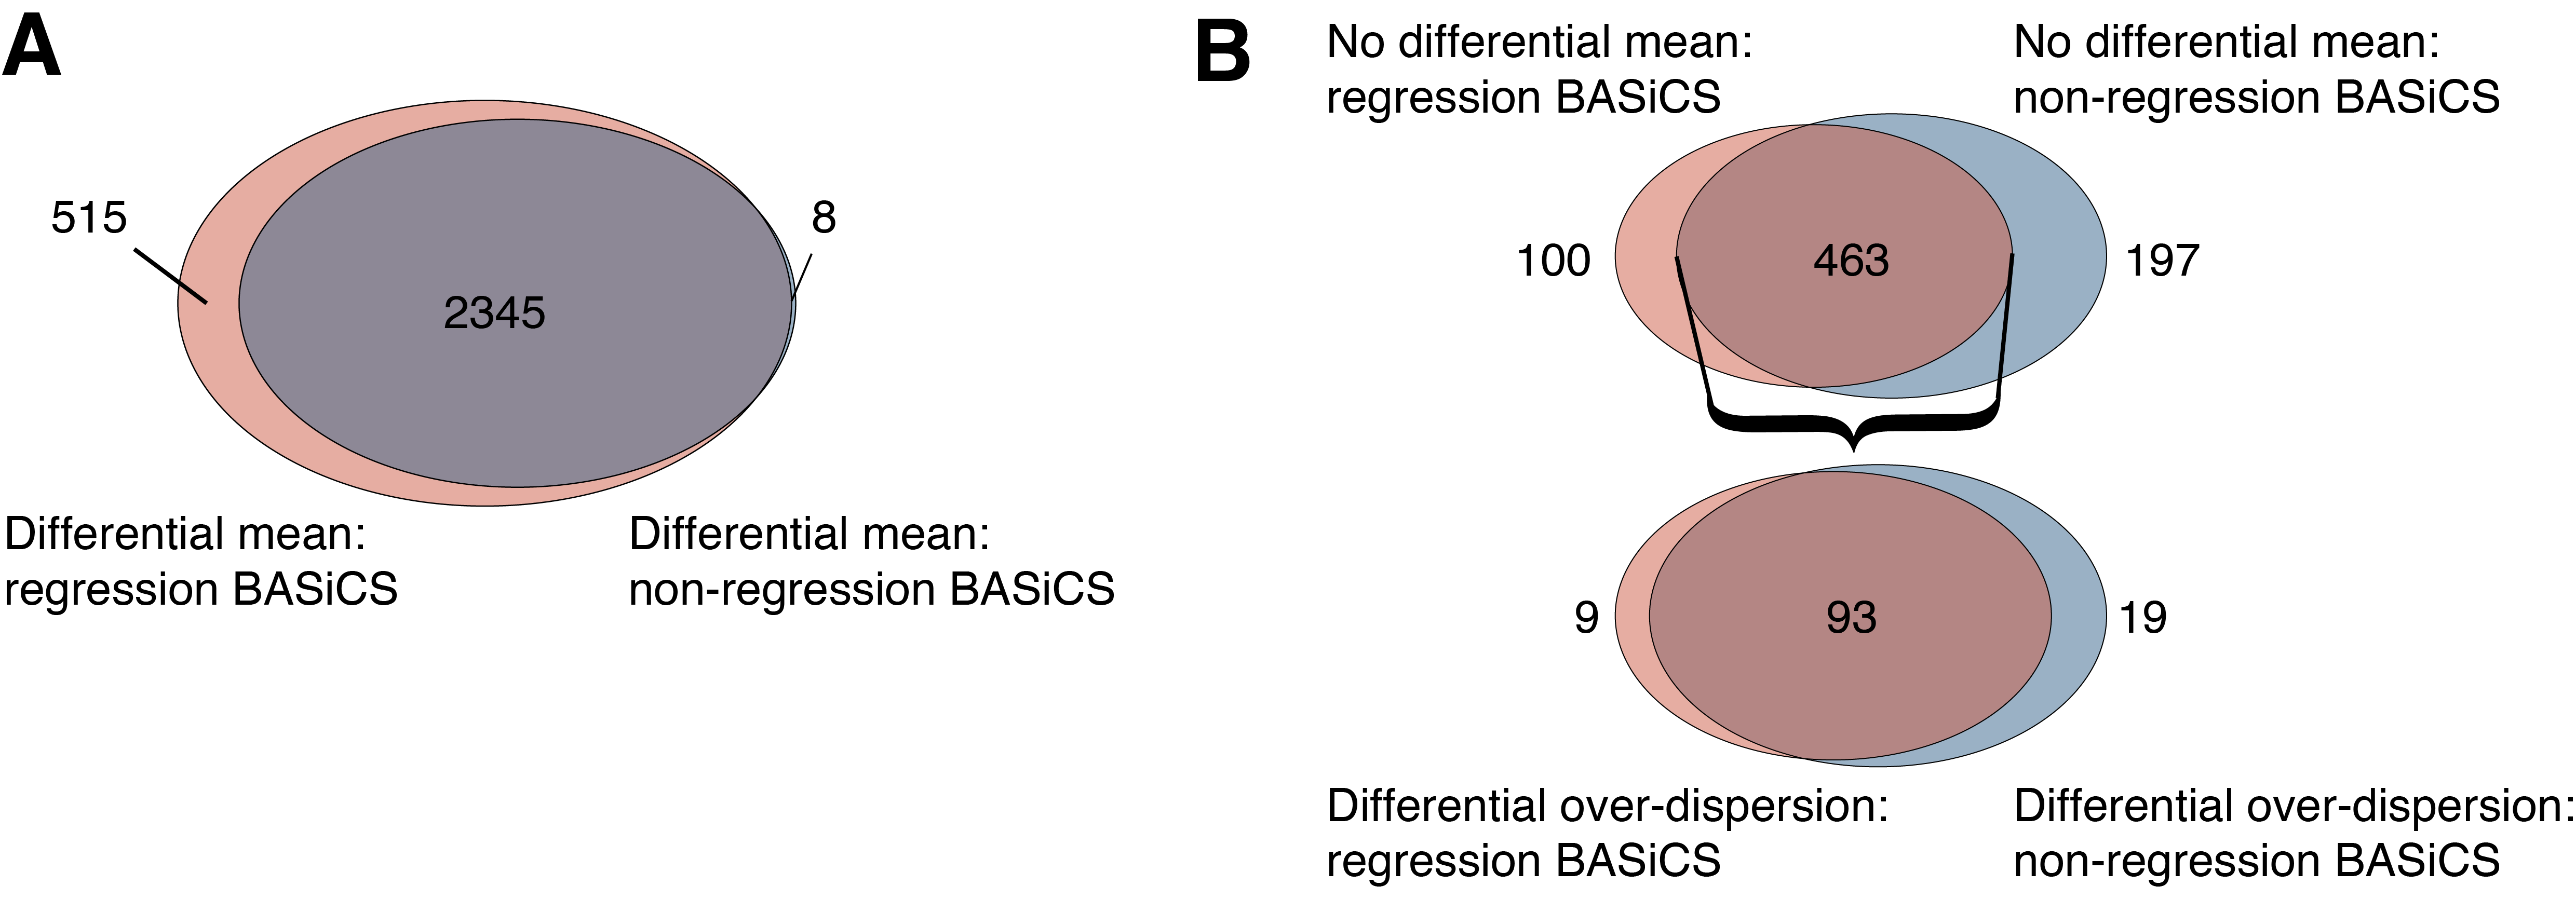
\includegraphics[width=\textwidth]{Fig_9.png}
\caption[Changes in transcriptional variability upon immune activation]{\textbf{Changes in transcriptional variability upon immune activation.}\\
\textbf{(A)} Genes up-regulated (red) and down-regulated (blue) by immune stimulation in young B6 mice. Non-differentially expressed genes shown in black. Average gene expression using posterior estimation, threshold of means > 50, log2FC > 2, FDR < 0.05; \textbf{(B)} Menes with no overall gene expression differences during activation (black dots in (A)) show decreased cell-to-cell variability in transcription (Mann-Whitney-Wilcoxon test, ***: p<10-10); \textbf{(C)} \textit{Eif1} is expressed in most cells in both conditions at similar levels, but shifts from stochastic to regulated expression; \textbf{(D)} To detect possible sub-populations in naive or activated CD4$^+$ T cells, differentially variable genes (log2FC > 0.4, FDR < 0.05) in naive cells with high gene-to-gene correlation (Spearman’s $\rho$ > 0.8) were used for hierarchical cluster analysis; \textbf{(E)} PCA of normalized counts of activated CD4$^+$ T cells from young B6 animals. PCA of activated CD4$^+$ T cells of young B6 animals after removing differences in the translation program as confounding factor.
}
\label{fig1:immune_variability}
\end{figure}

We next profiles changes in expression variability upon immune activation. Due to the strong confounding effect observed between mean expression and variability estimates, we only profiled genes that show no changes in mean expression between the naive and activated state (see \textbf{Box 2},indicated as black dots in \textbf{Fig. \ref{fig1:immune_variability}A}, log2FC = 0, FDR < 0.05). We observed a significant reduction in cell-to-cell transcriptional variability among genes whose transcription levels do not change after activation (Mann-Whitney-Wilcoxon test, p<10-10) \textbf{(Fig. \ref{fig1:immune_variability}B)}. For example, the eukaryotic translation initiation factor 1 (Eif1), show a marked decrease in cell-to-cell transcriptional variability, consistent with increased regulatory coordination \textbf{(Fig. \ref{fig1:immune_variability}C)}.To investigate whether genes that are more variably expressed in the naive than the activated condition showed coordinated patterns of expression potentially associated with cryptic substructure, we identified genes with statistically higher expression variability in the naive population compared to activated cells (variability log2FC > 0.4, FDR < 0.05, no change in mean expression). Genes with high variability and high pairwise correlation (Spearman’s rho > 0.8) in the naive population can be used to identify possible sub-populations of CD4$^+$ T cells. A hierarchical clustering analysis did not show any signs of this substructure \textbf{(Fig. \ref{fig1:immune_variability}D)}. 

\begin{figure}[!ht]
\centering
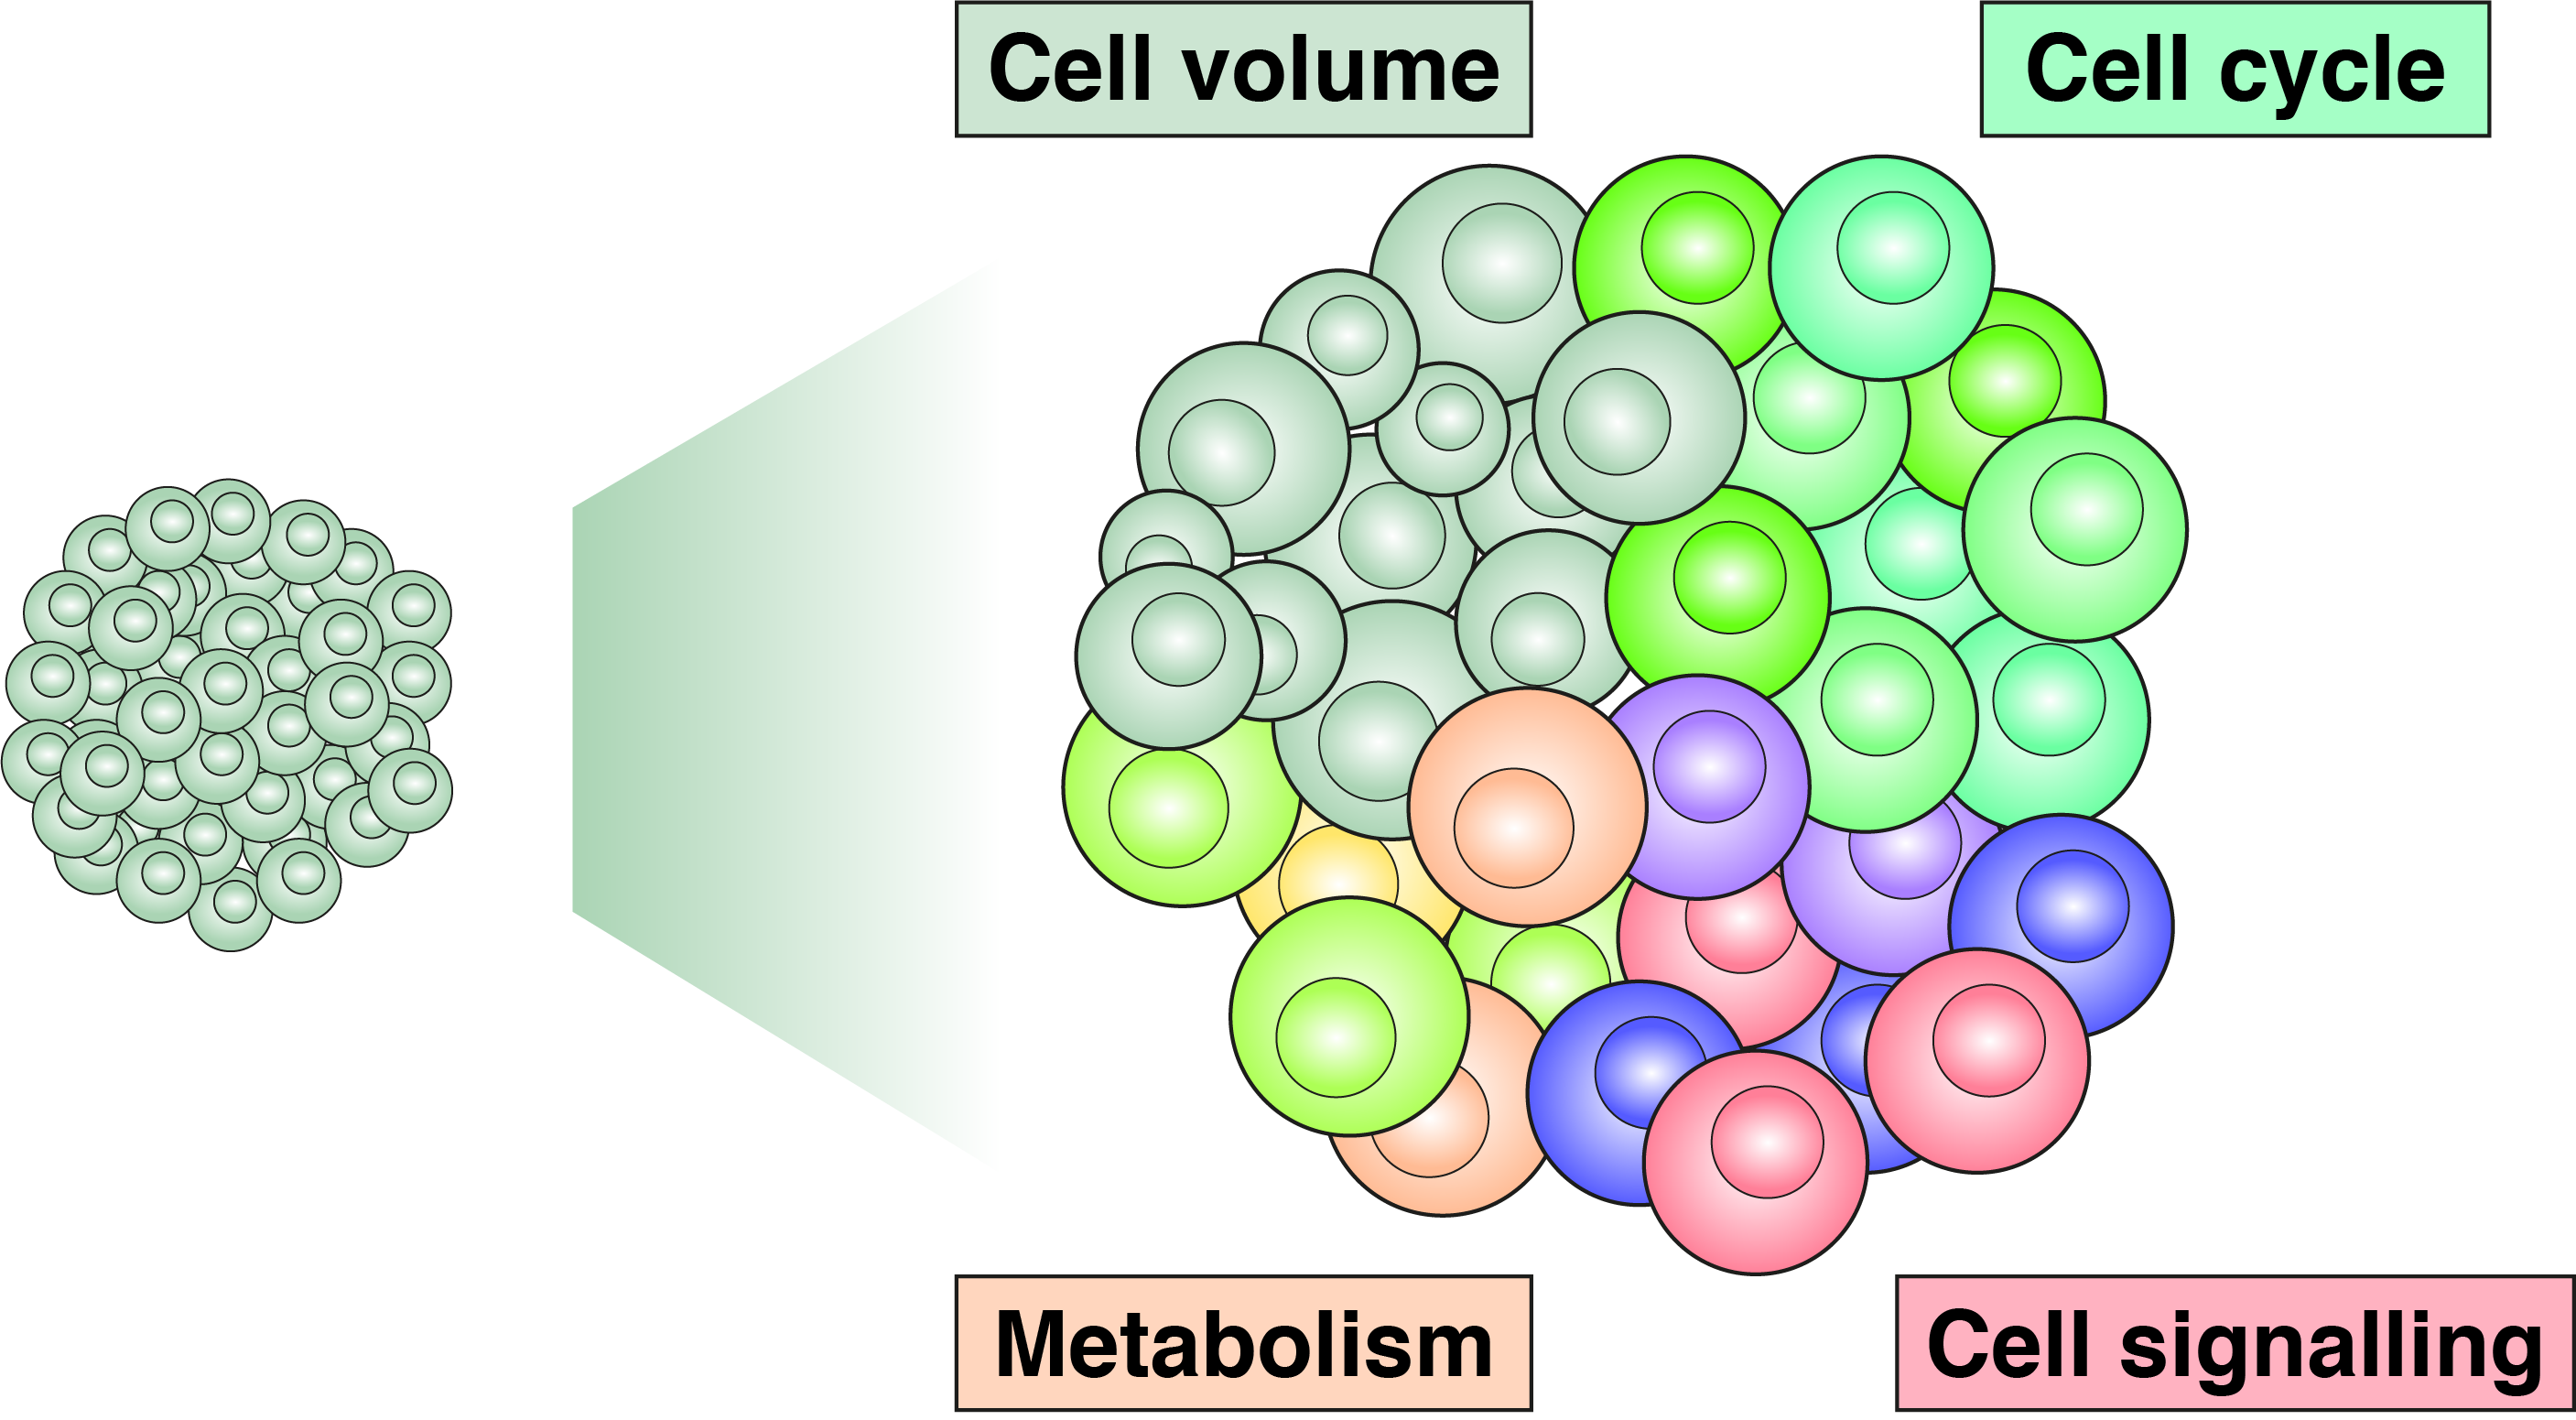
\includegraphics[width=0.7\textwidth]{Fig_10.png}
\caption[Immune activation dynamics in young CAST animals]{\textbf{Immune activation dynamics in young CAST animals.}\\
\textbf{(A)} Activation of CD4$^+$ T cells from young CAST mice in anti-CD3$\epsilon$/CD28 coated plates induces large-scale transcriptional changes, visualized using tSNE dimensionality reduction; \textbf{(B)} Genes up-regulated (red) and down-regulated (blue) by immune stimulation in young CAST mice. Non-differentially expressed genes used in (C) are shown  in black. Average gene expression using posterior estimation, threshold of means > 50, log2FC > 2, FDR < 0.05; \textbf{(C)} Genes with no overall gene expression differences during activation show decreased cell-to-cell variability in transcription (Mann-Whitney-Wilcoxon test, ***: p<10-10); \textbf{(D)} Up-regulated genes were expressed in a relatively large fraction of activated CD4$^+$ T cells after stimulation (median 25\%); down-regulated genes were expressed in a smaller fraction of naive CD4+ T cells (median 17\%). 600 genes of each condition were randomly selected.
}
\label{fig1:immune_activation_CAST}
\end{figure}

Finally, it has been observed that covariance between cells due to unobserved factors such as the cell cycle can mask potentially interesting biological signals \citep{Stegle2015}. In our dataset, ribosomal biogenesis is the strongest mediator of CD4$^+$ T cell function upon activation. Importantly, controlling for this factor using scLVM \citep{Buettner2015} and re-performing the analysis on the corrected data did not reveal concealed cellular processes \textbf{(Fig. \ref{fig1:immune_variability}E)}.\\

In sum, activation of CD4+ T cells drives a transcriptional switch that alters the global expression profile from a stochastic to a tightly regulated state. To test whether these transcriptional dynamics are evolutionarily conserved, we performed the same analysis for CD4$^+$ T cells extracted from CAST and detect similar activation dynamics \textbf{(Fig. \ref{fig1:immune_activation_CAST})}.



In sum, activation of CD4+ T cells drives a transcriptional switch that alters the global expression profile from a stochastic to a tightly regulated state. To test whether these transcriptional dynamics are evolutionarily conserved, we performed the same analysis for CD4$^+$ T cells extracted from CAST and detect similar activation dynamics \textbf{(Fig. \ref{fig1:immune_activation_CAST})}.

\section{Conservation of CD4$^+$ T cell activation}
\subsection*{The core activation process is highly conserved in divergent mouse species}

We detect similar activation patterns when comparing CD4$^+$ T cell activation between B6 and CAST. To further study the conservation of the immune response, we used the rapid divergence in gene expression between CD4$^+$ T cells in B6 and CAST to refine the functional targets activated upon immune stimulation \citep{Shay2013}. We reasoned that such targets would be both conserved between species and expressed in most cells, whereas the genes activated species-specifically would be less likely to be functional targets and more likely to be sporadically expressed.\\

\begin{figure}[!ht]
\centering
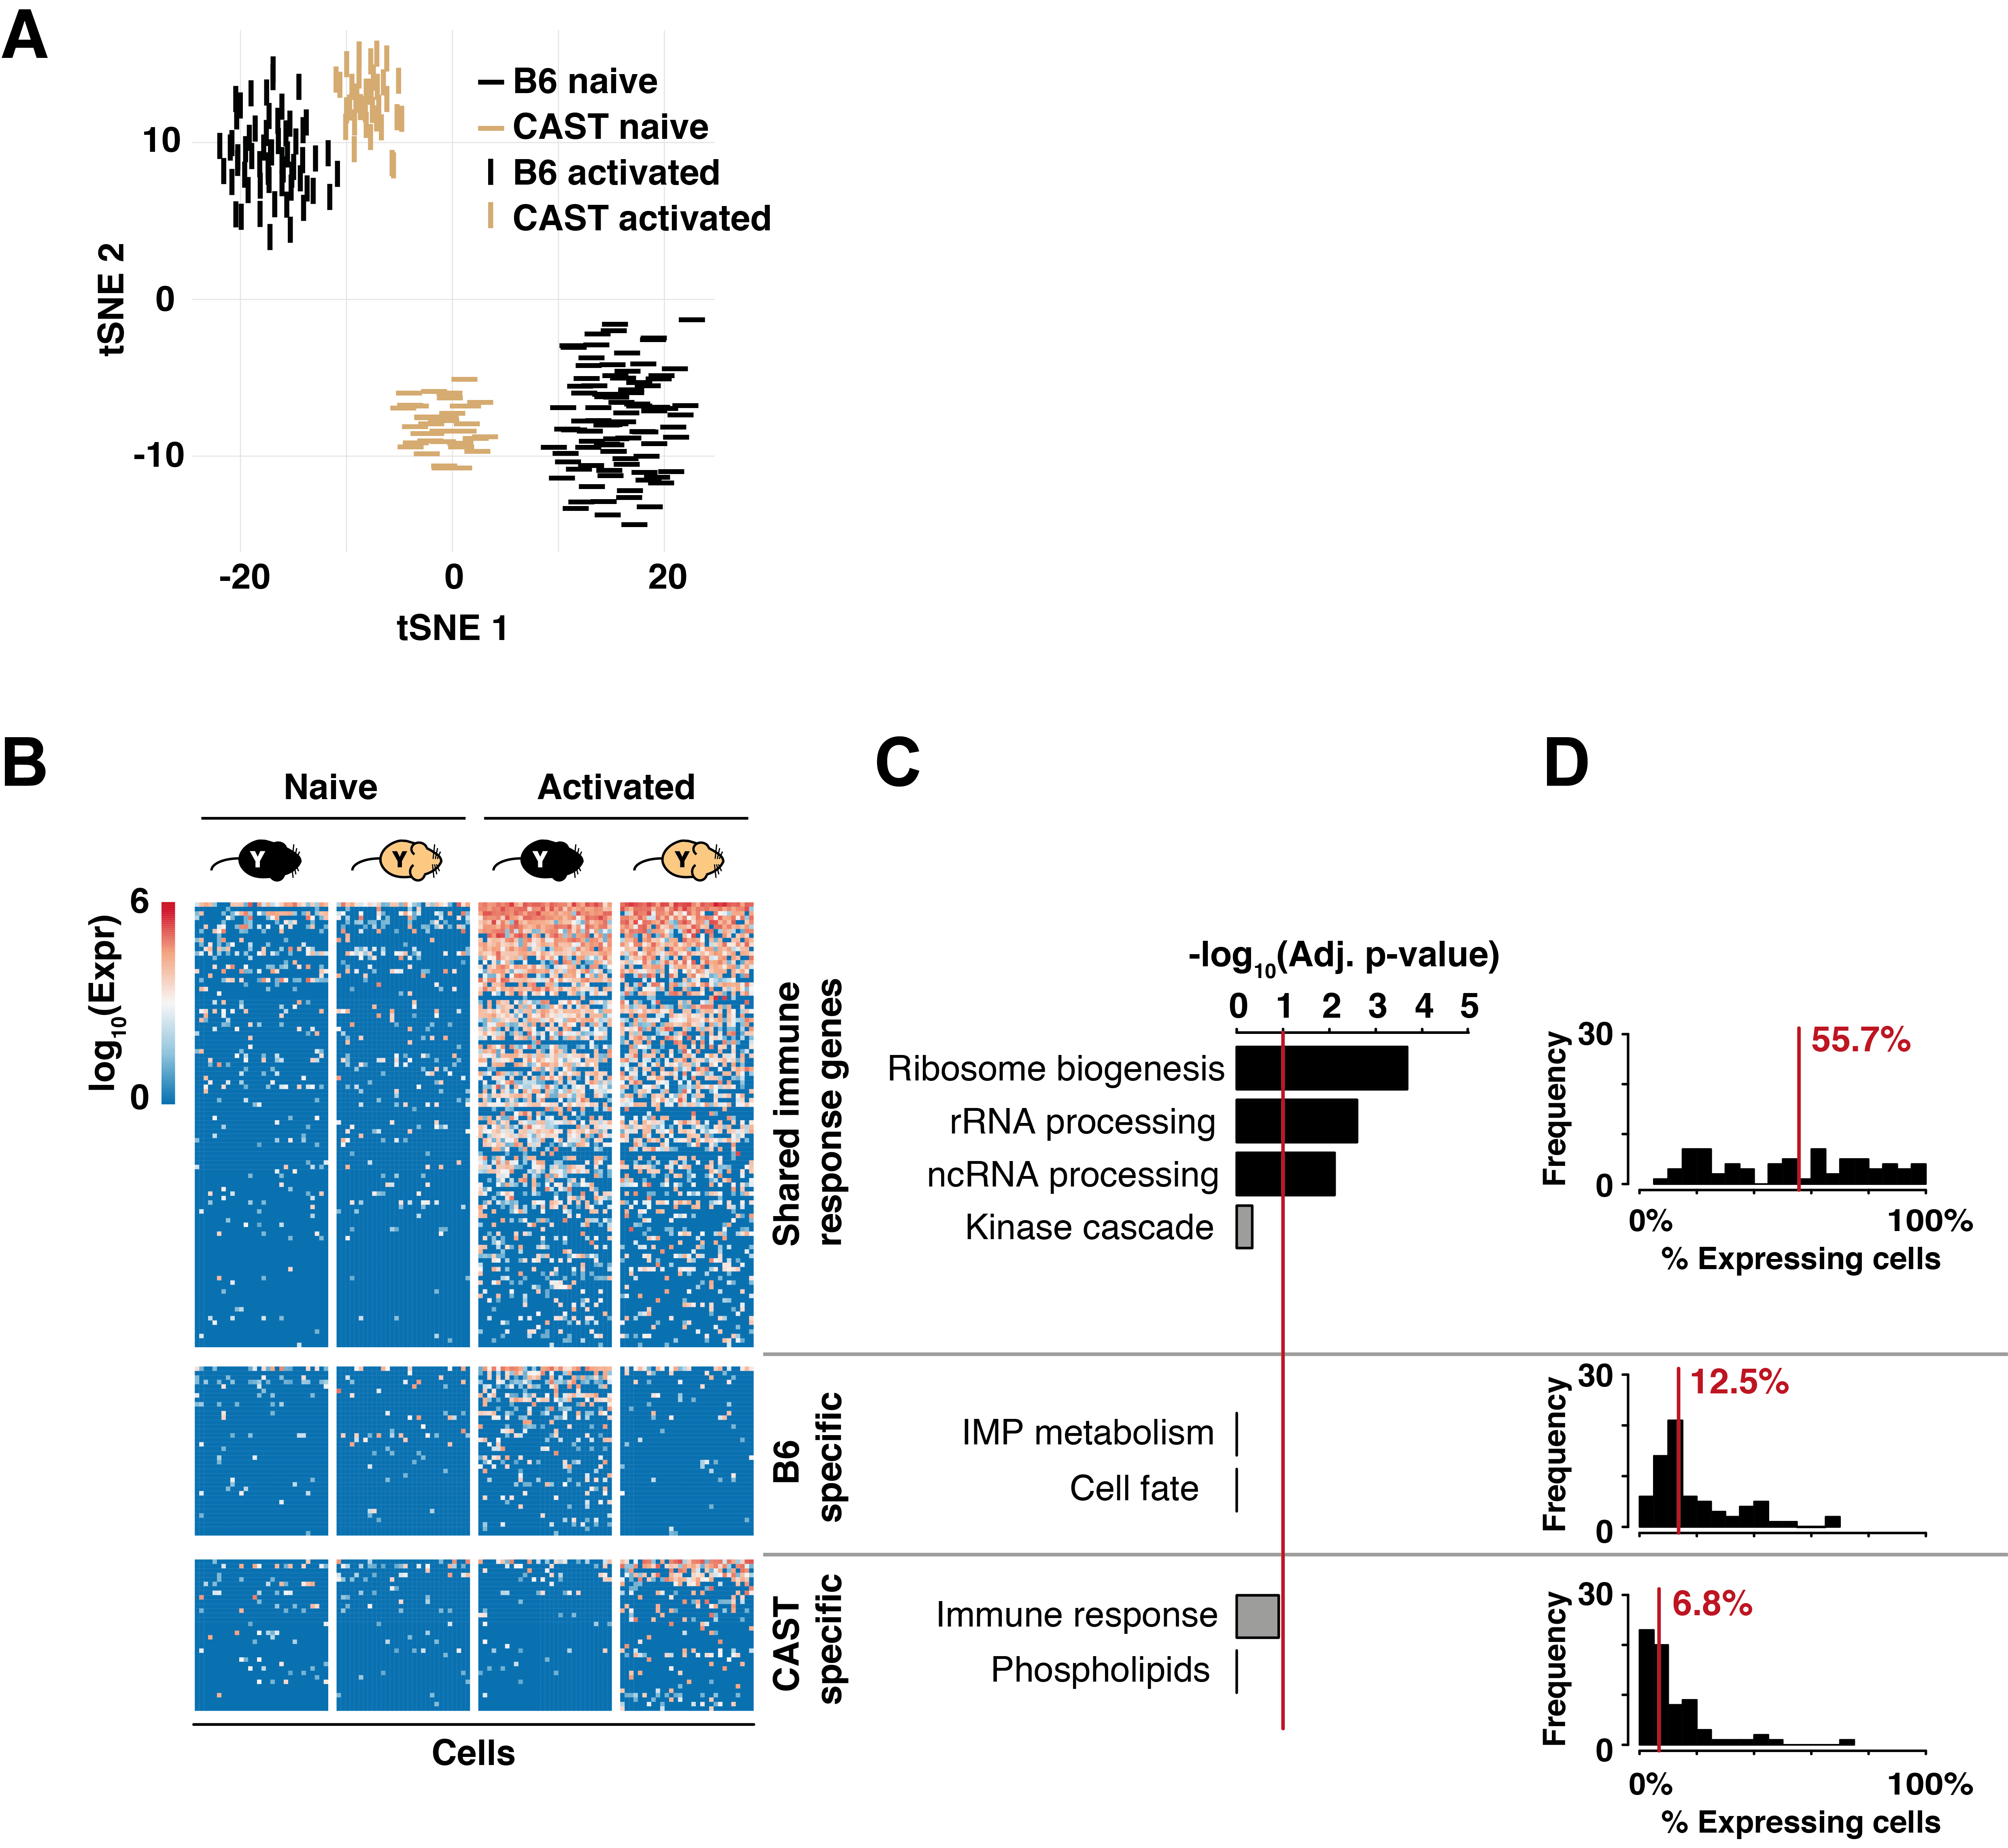
\includegraphics[width=0.9\textwidth]{Fig_11.png}
\caption[Shared CD4$^+$ T cell activation programme]{\textbf{Shared CD4$^+$ T cell activation programme.}\\
\textbf{(A)} CD4$^+$ T cells isolated from B6 (black) and CAST (orange) show similar large-scale transcriptional changes upon immune stimulation; \textbf{(B)} Immune activation of CD4$^+$ T cells trigger up-regulation of both conserved (upper panel), and species-specific (lower panels) transcriptional programs. For visualization purposes, genes in shared and species-specific categories were proportionately and randomly selected. 30 cells were randomly selected for each condition/species; \textbf{(C)} Genes up-regulated in both B6 and CAST highly enrich for known T cell functionality; genes up-regulated in only B6 or CAST have no statistically significant functional enrichment (Bonferroni multiple testing corrected p-values, red line is 0.1); \textbf{(D)} Fractions of cells in which a gene is detected are displayed as histograms; 70 genes were randomly selected from each gene set. While most genes in the shared activation process are expressed in a high percentage of cells, only few cells express species-specific genes of the activation process.}
\label{fig1:shared_activation}
\end{figure}


As described for B6 above, we stimulated naive CD4$^+$ T cells isolated from young CAST males using anti-CD3$\epsilon$/anti-CD28 antibodies followed by scRNAseq \textbf{(Fig. \ref{fig1:shared_activation}A)}. To find genes that form the evolutionarily conserved, core activation program, we test for differential expression between the naive and activated state separately in B6 and CAST (log2FC > 2, FDR < 0.05). Genes that are up-regulated after activation similarly in B6 and CAST form the shared activation program. Up-regulated genes that are differentially expressed in activated cells between the two species form the set of species-specific response genes; differential expression analysis was performed on genes up-regulated in either B6 or CAST (log2FC > 2, FDR < 0.05). To identify the set of species-specific response genes that might be caused by mapping artifacts, we quantified gene expression in activated CAST and B6 samples based on the CAST and GRCm38 genome as described above. Genes in the activated state that show differential mapping between the two genomes were excluded from the species-specific lists of response genes. We find 225 genes strongly up-regulated similarly in B6 and CAST while 1208 genes in total are up-regulated across both species. Out of these genes, 171 are detected as differentially expressed between the two species forming the set of species-specific genes. For visualization purposes, we randomly selected 100 out of the 225 shared response genes, 43 of the 96 B6 specific and 33 of the 75 CAST specific response genes \textbf{(Fig. \ref{fig1:shared_activation}B)}.\\

The set of shared genes was strongly enriched for cellular processes known to be immediately activated by stimulation of CD4$^+$ T cells, including the core translational machinery (ribosome biogenesis and rRNAs, \textbf{Fig. \ref{fig1:shared_activation}C}) and key immune activation genes (such as Il2ra and Tnfrsf9)\citep{Asmal2003}. Genes up-regulated after activation were expressed across most CD4+ T cells in both B6 and CAST. In contrast, species-specific genes (96 for B6, 75 for CAST) showed no enrichment for biological function \textbf{(Fig. \ref{fig1:shared_activation}C)}. While most shared response genes are expressed across the whole cell populations, species-specific response genes tend to be expressed in only a small fraction of cells \textbf{(Fig. \ref{fig1:shared_activation}D)}. \\

Our interspecies comparison thus revealed that target genes involved in translational control and immune function represent the conserved signature within the early activation response.

\newpage

\section{Destabilization of CD4$^+$ T cell activation during ageing}
\subsection*{The core activation program becomes destabilized during ageing}

Ageing can cause perturbation of cell cycle entry for hematopoietic stem cells, leading to a shift in the functional balance between self-renewal and differentiation \citep{Kowalczyk2015}. We considered whether ageing might similarly perturb the transcriptional response of CD4$^+$ T cells to immune stimulation. By comparing the activation responses between different sub-species of mice, we could also establish whether any observed impact of ageing is conserved.\\

We firstly asked whether the overall response of CD4$^+$ T cells is perturbed during ageing and compared mean expression of cells isolated from young and old mice. Principal component analysis revealed that the global expression profiles of naive or activated CD4$^+$ T cells did not change due to ageing \textbf{(Fig. \ref{fig1:mean_expression_ageing}A and B)}. For each species, we identified differentially expressed genes between young and old animals separately for naive and activated CD4$^+$ T cells \textbf{(Fig. \ref{fig1:mean_expression_ageing}C and D)}. Only around 15\% of all tested genes showed changes in mean expression between you and old animals. Additionally, these genes showed low expression in naive or activated cells taken from young and old animals. To further quantify this, we computed the fraction of cells in which each differentially expressed gene was expressed. The distribution of these values was added as inlets to the plots (x-axis ranging from 0\% to 100\% of cells) and showed and enrichment for genes that are expressed in only subset of cells. This indicates that changes in mean expression during ageing only affect lowly expressed genes that are detected only in subsets of cells. These effects can also arise due to increased levels of noise for lowly expressed genes. \\

To test whether these subtle effects during ageing are shared between the two species, we calculated the Jaccard index, which measures the overlap between sets of elements, separately for up- and down-regulated genes \textbf{(Fig. \ref{fig1:mean_expression_ageing}E and F)}. We only detect $\sim$3\% of differentially expressed genes as being shared between the two species. Therefore, we did not find a conserved ageing signature that affects expression levels in CD4$^+$ T cells.

\newpage

\begin{figure}[!ht]
\centering
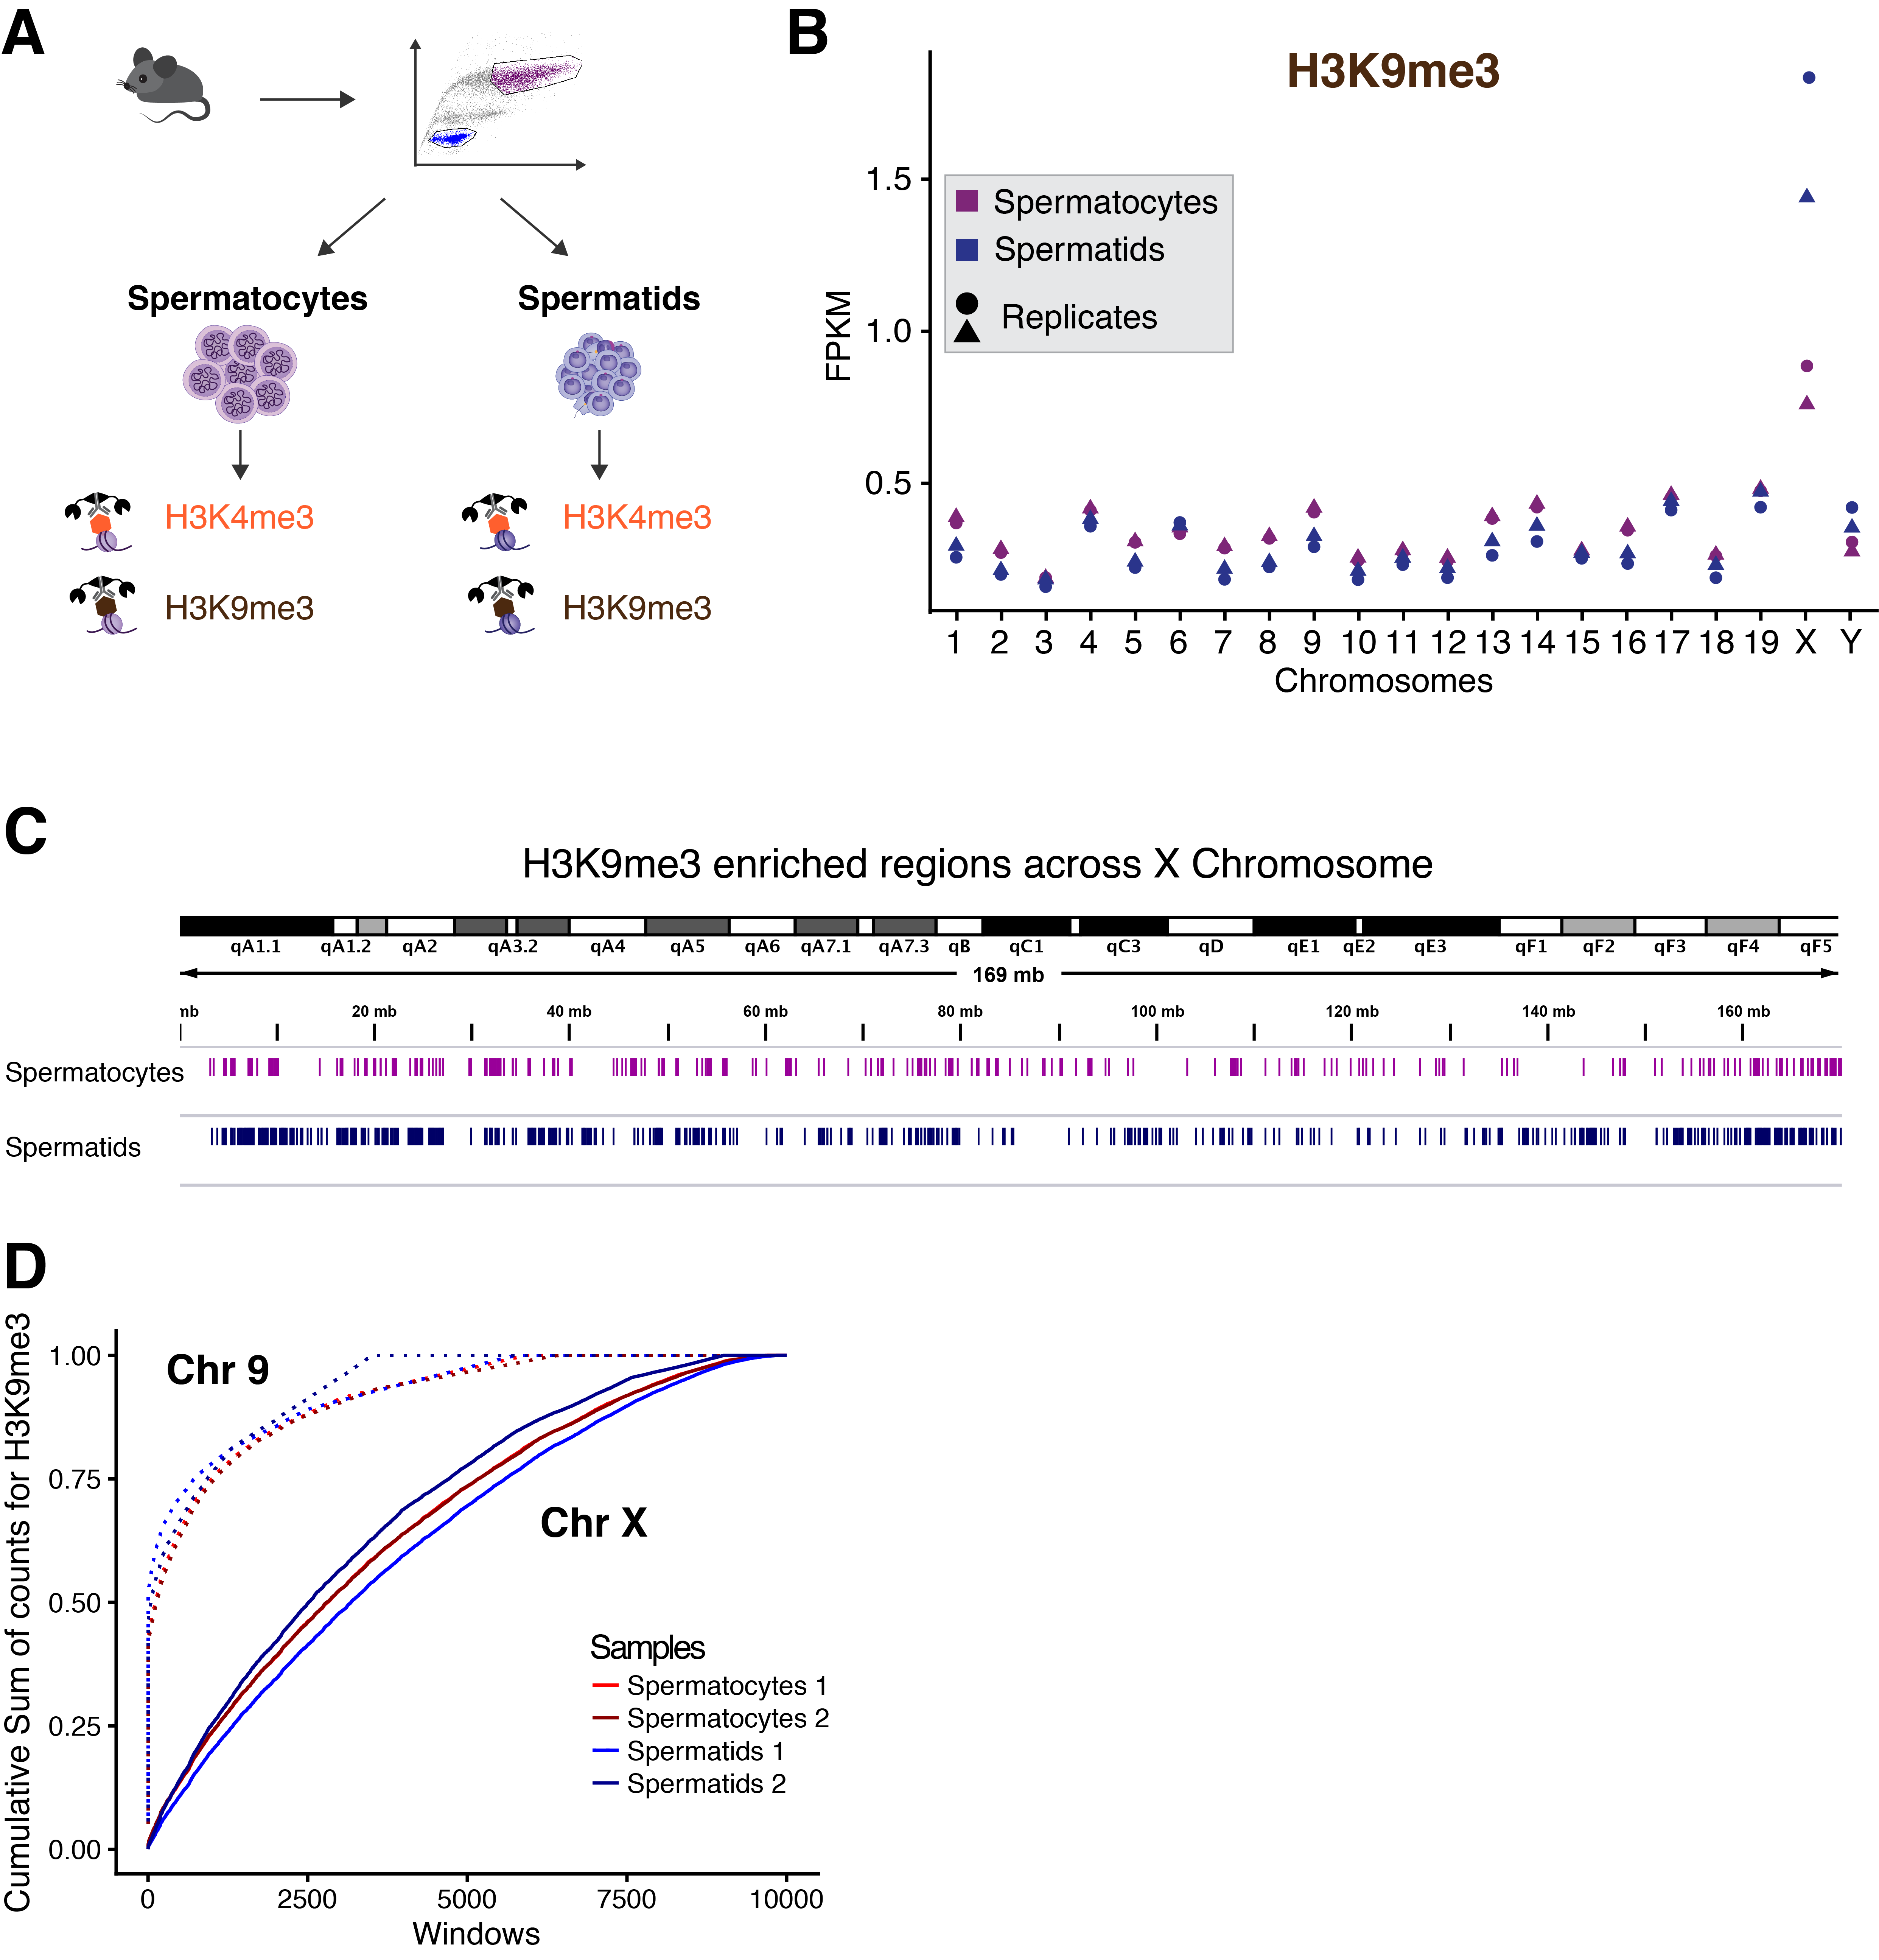
\includegraphics[width=0.9\textwidth]{Fig_12.png}
\caption[Global immune response during ageing]{\textbf{Aging did not change the global expression profile of naive or activated CD4$^+$ T cells (full legend on next page).}}
\label{fig1:mean_expression_ageing}
\end{figure}

\newpage

\captionsetup[figure]{list=no}
\addtocounter{figure}{-1}   
\captionof{figure}{\textbf{Aging did not change the global expression profile of naive or activated CD4$^+$ T cells (continued).}\\
Principal component analysis reveals no separation between cells isolated from young or old animals in the naive \textbf{(A)} or activated \textbf{(B)} state; \textbf{(C)} 7.1\% of all tested genes in B6 and 10.3\% of genes in CAST are differentially expressed in naive CD4$^+$ T cells between old (red) and young (blue) animals. Average gene expression using posterior estimation, threshold of means > 50, log2FC > 2, FDR < 0.05. Insets show distributions of fraction of cells in which these genes are expressed. X-axis: 0\% - 100\% of cells;  \textbf{(D)} 10\% of all tested genes in B6 and 9\% of genes in CAST are differentially expressed in activated CD4$^+$ T cells between old (red) and young (blue) animals. Average gene expression using posterior estimation, threshold of means > 50, log2FC > 2, FDR < 0.05. Insets show distributions of fraction of cells in which these genes are expressed. X-axis: 0\% - 100\% of cells; \textbf{(E)} The overlap of ageing-associated genes in naive cells was calculated using the Jaccard index between gene sets. Genes highly expressed in old animals (red) or genes highly expressed in young animals (blue) show little overlap (3\%) between B6 and CAST; \textbf{(F)} The overlap of ageing-associated genes in activated cells was calculated using the Jaccard index between gene sets. Genes highly expressed in old animals (red) or genes highly expressed in young animals (blue) show little overlap (2-3\%) between B6 and CAST.
\\}
\captionsetup[figure]{list=yes}

We next focused on the conserved activation program in activated CD4$^+$ T cells. Consistent with the findings from analysis changes in global expression between young and old animals,  the majority of genes in the core program responded upon stimulation, irrespective of age \textbf{(Fig. \ref{fig1:variability_ageing}A)}. We then profiled the change in mean expression of activated cells between young and old animals and detected the magnitude of the activation response to be consistently reduced in older mice in both species \textbf{(Fig. \ref{fig1:variability_ageing}B)}. When considering genes with no changes in mean expression (see \textbf{Box 2}), we observe an increase in cell-to-cell transcriptional variability of the core activation program in older animals compared to young animals \textbf{(Fig. \ref{fig1:variability_ageing}C)}. We next asked for the driver of the increase in transcriptional variability during ageing. Therefore, we calculated the fraction of cells in which genes of the shared activation program are expressed and compared these fractions between activated cells isolated from old or young animals in both species. We used a binomial test to evaluate which genes significantly change the percentage of cells expressing these genes (Bonferroni corrected p-values < 0.1). Gene expression in activated cells isolated from old animals was used as the Null-distribution \textbf{(Fig. \ref{fig1:variability_ageing}D)}. \\

These results indicate a destabilization of the immune response programme during ageing. While most response genes are expressed to similar levels in activated cells of young and old animals, we detect a subset of cells loosing the expression of these genes in aged mice. These dropouts in expression do not correlate across the population of cells and appear to be more stochastic.

\newpage

\begin{figure}[!ht]
\centering
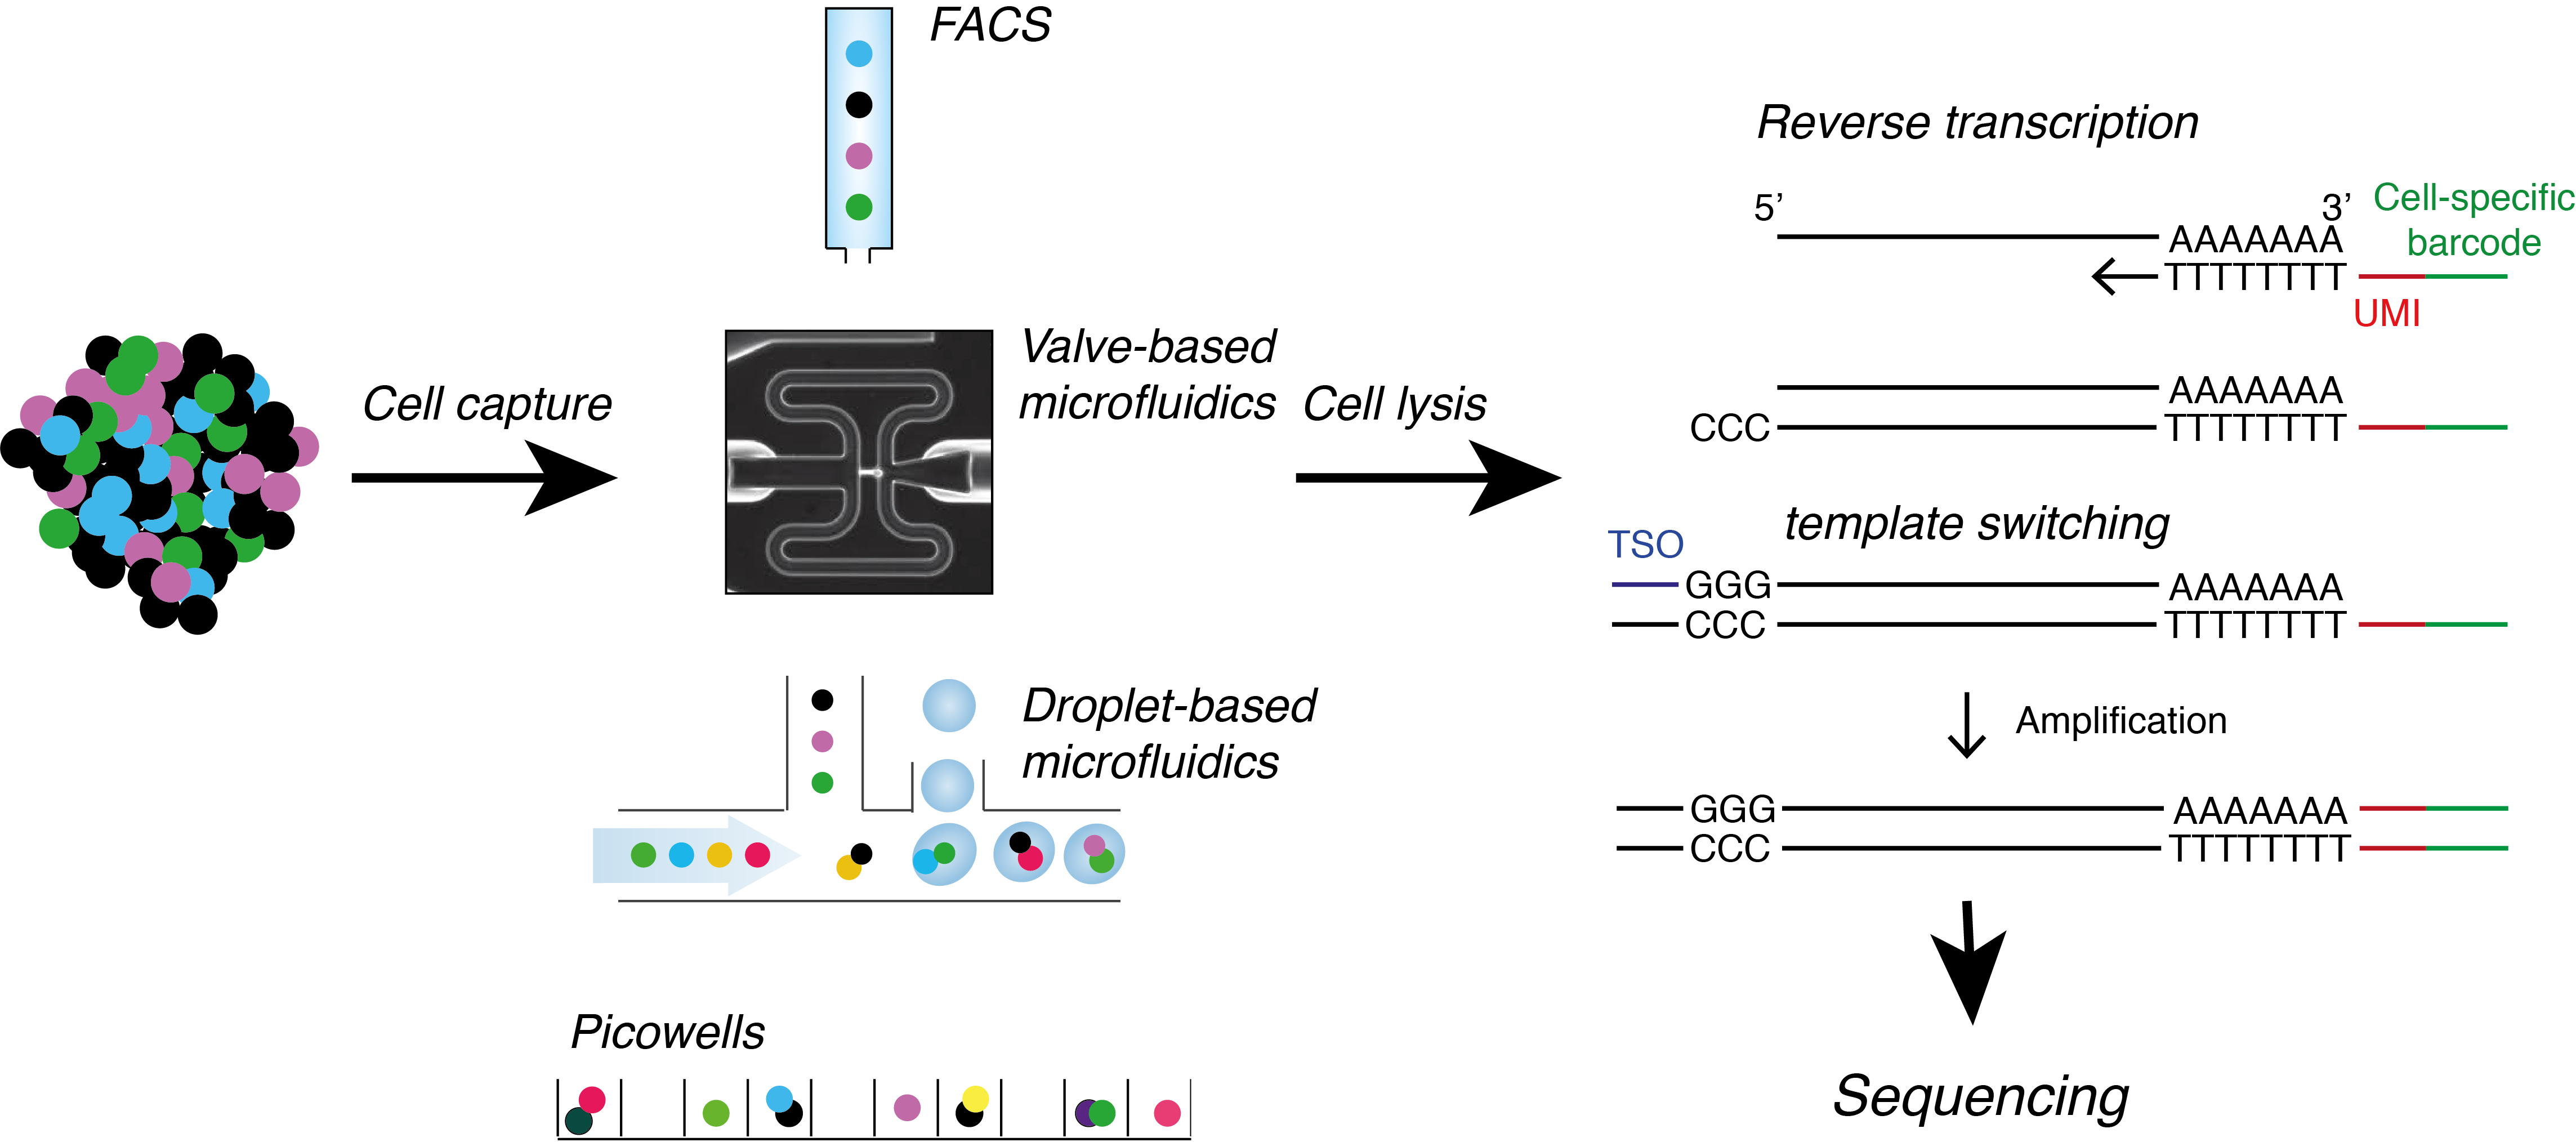
\includegraphics[width=\textwidth]{Fig_13.png}
\caption[Ageing destabilizes the CD4$^+$ T cell response]{\textbf{Ageing counteracts the decrease in cell-to-cell variability needed during early activation of CD4$^+$ T cells.} \\
\textbf{(A)} Full heatmap showing all 225 genes of the shared activation program expressed in all activated cells from young and old CAST and B6. Genes were ordered based on their mean expression; \textbf{(B)} Fold changes in mean expression indicate a consistent trend in lower expression of the shared activation program in cells from old animals (genes were ordered by mean expression, log2FC of posterior mean estimates); \textbf{(C)} Cells from old animals show higher transcriptional variability compared to young animals (genes were ordered by mean expression, log2FC of posterior over-dispersion estimates); \textbf{(D)} The fraction of cells in which genes of the shared activation process are expressed is reduced in CD4$^+$ T cells from old animals. The distribution of fraction values is plotted on each corresponding axis (medians of fraction values are indicated in red); changes in fraction values were tested using a binomial test.}
\label{fig1:variability_ageing}
\end{figure}

We next asked whether the increase in variability is driven by technical factors and hidden sub-structure within the data. Therefore, we generated independent replicates of naive and activated CD4$^+$ T cells from young and old B6 animals using Fluidigm C1 machines at a different research institute. Profiling changes in variability using these biological replicates, we confirmed the increase in transcriptional variability during aging \textbf{(Fig. \ref{fig1:validation}A)}.

\begin{figure}[!ht]
\centering
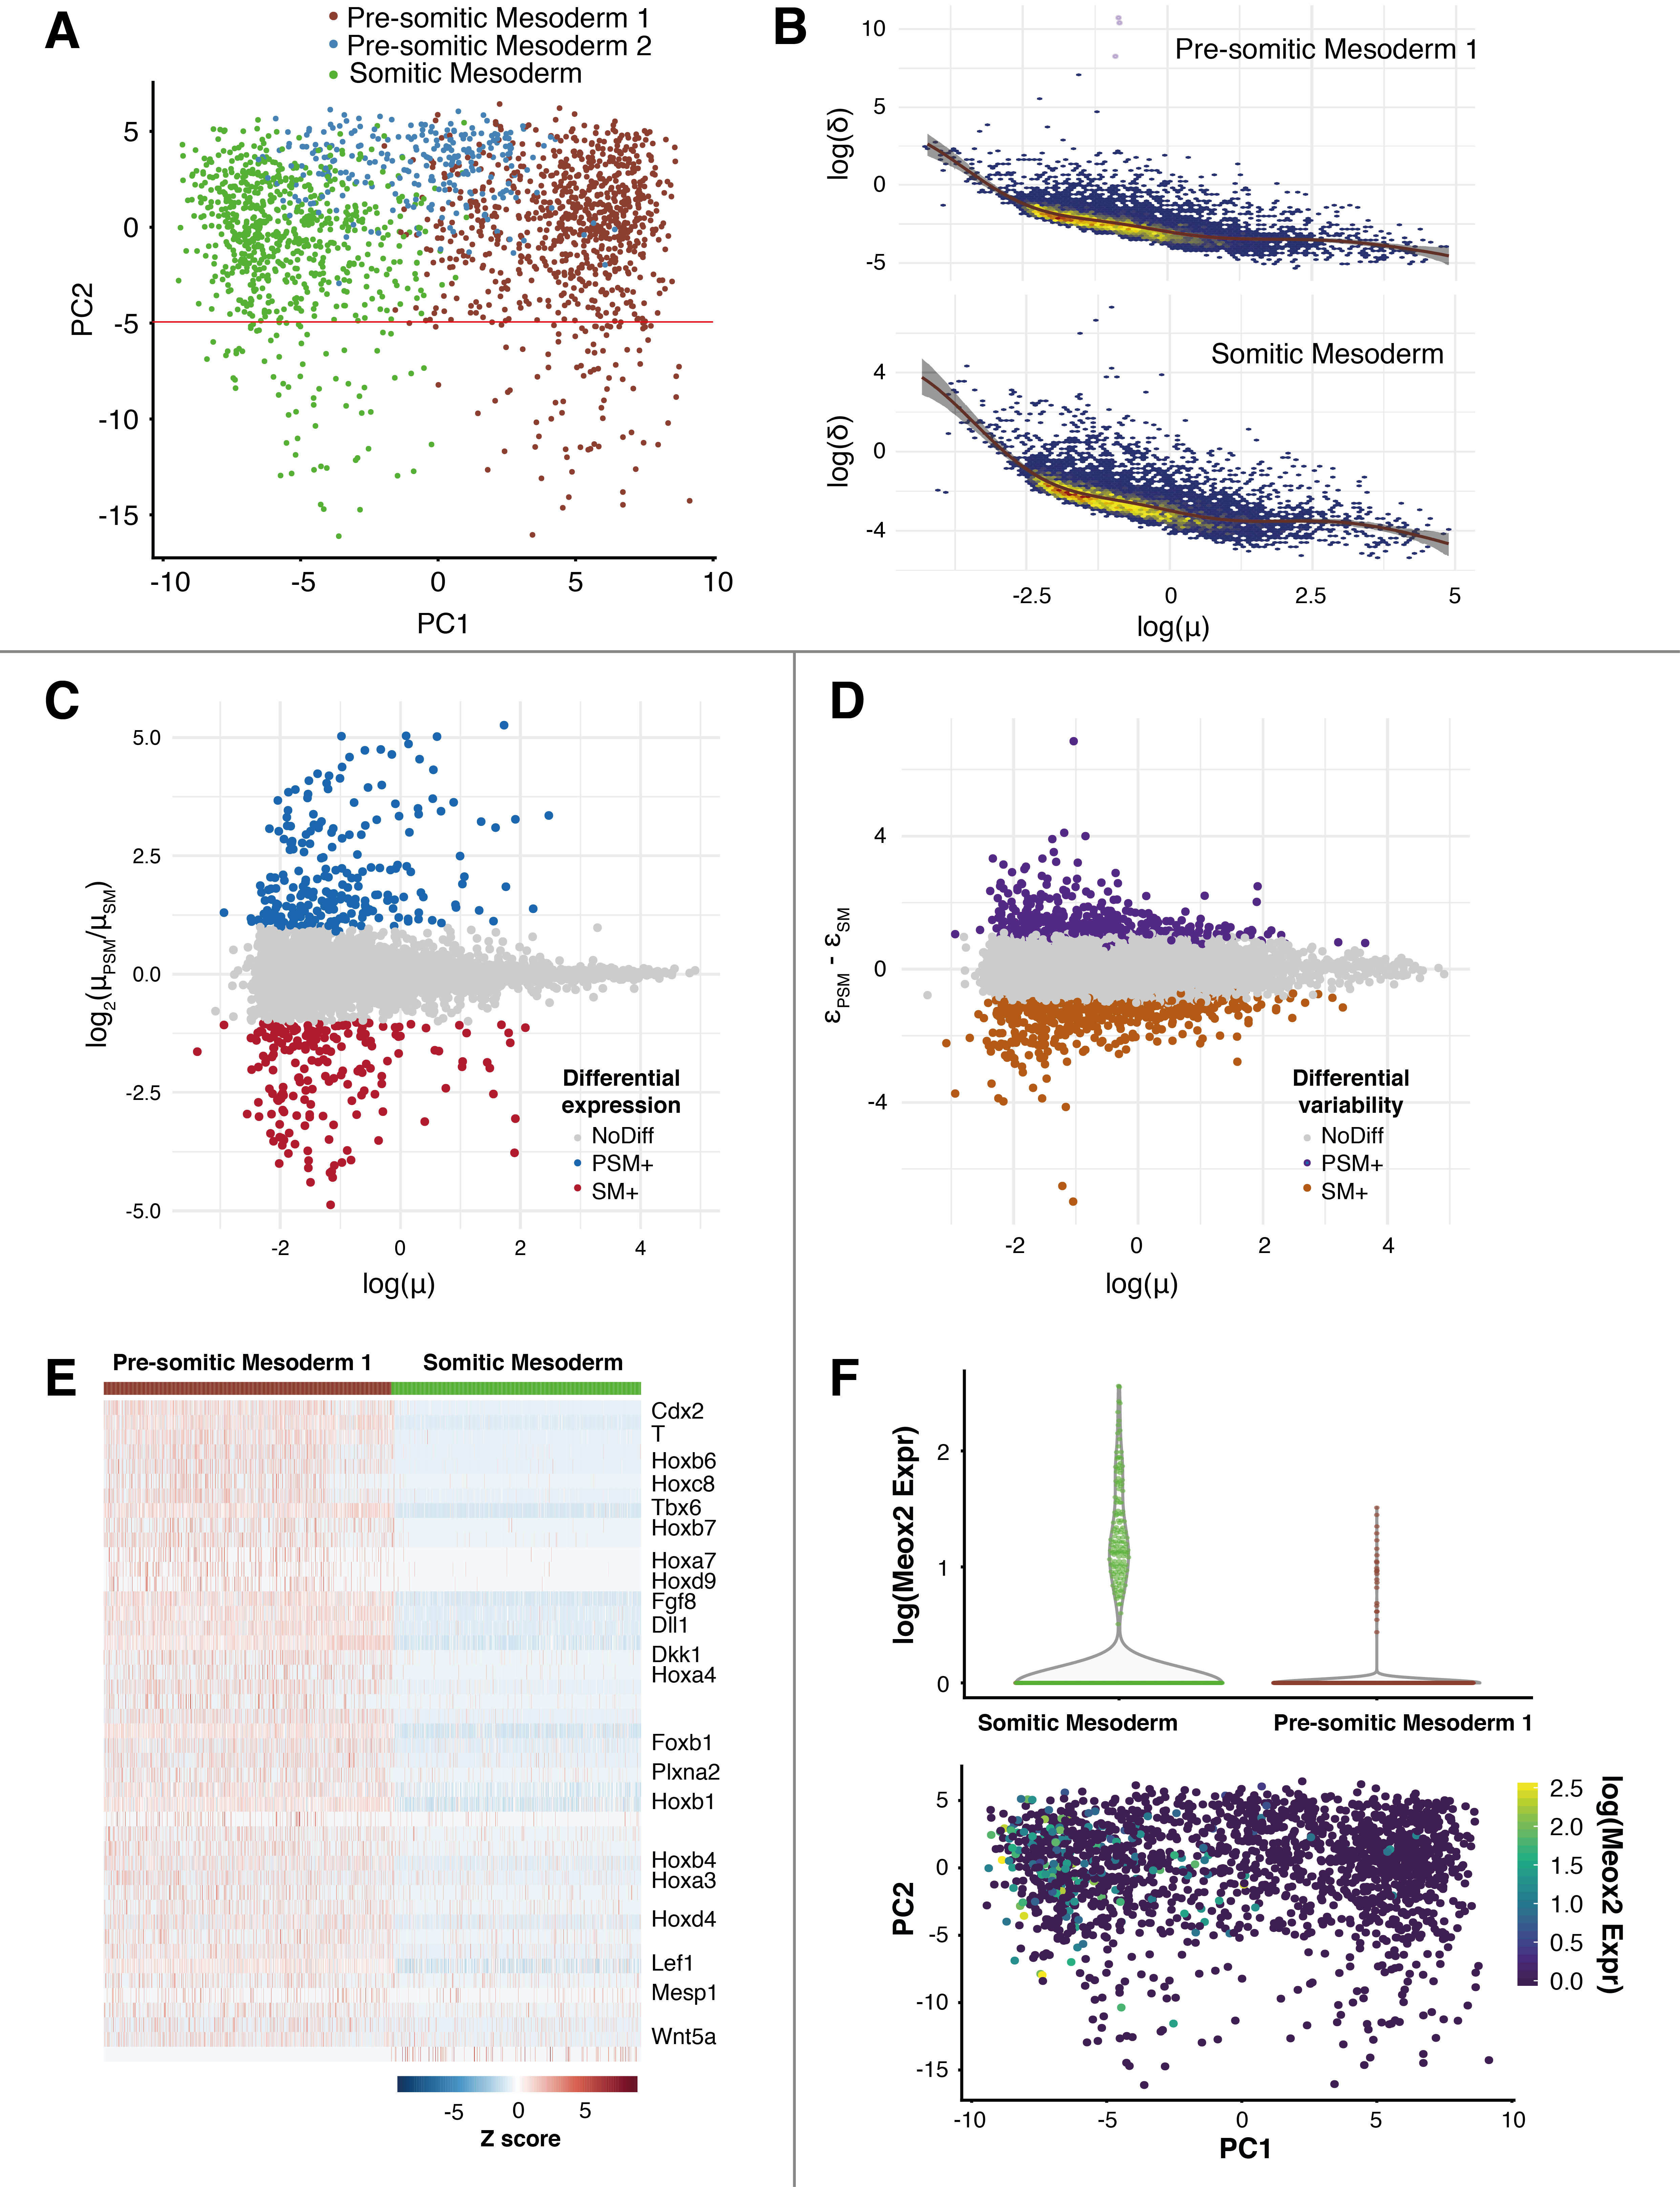
\includegraphics[width=\textwidth]{Fig_14.png}
\caption[Experimental validation of increased transcriptional variability during ageing]{\textbf{Experimental validation of increased transcriptional variability during ageing.} \\
\textbf{(A)} A biological replicate of 115 activated CD4$^+$ T cells from old B6 animals was generated and changes in gene expression variability were compared to activated CD4$^+$ T cells from young B6 animals; \textbf{(B)} 30 out of all activated CD4$^+$ T cells from young or old B6 mice were randomly selected and changes in gene expression variability were compared between the downsampled populations of cells; \textbf{(C)} Expression of CD4$^+$ T cell activation markers in all activated cells from young and old B6 before (left) and after (right) filtering based on \textit{Ifng}, \textit{Sell}, \textit{Trac}, \textit{Il2ra} and \textit{Cd69} expression; \textbf{(D)} Changes in gene expression variability of activated cells between young and old animals are displayed before (left) and after (right) filtering (see (C)).}
\label{fig1:validation}
\end{figure}

Since quantification of transcriptional variability can be biased based on the number of cells present in each cell population, we downsampled both young and old activated CD4$^+$ T cells and detected the same increase in variability during ageing \textbf{(Fig. \ref{fig1:validation}B)} as previously when comparing the full set of CD4$^+$ T cells \textbf{(Fig. \ref{fig1:variability_ageing}C)}. Next, we tested whether the global shift in variability is caused by different cell population structures between old and young B6 animals and removed cells expressing marker genes that were inconsistent with their activation state as well as cells with a possible Th1 differentiation bias (\textit{Ifng} expressing). Based on the library size adjusted counts, we removed activated cells with low \textit{Cd69} (< 300 counts), high \textit{Sell} (> 10 counts), low \textit{Trac} (< 100 counts), low \textit{Il2ra} (< 100 counts) and \textit{Ifng} (> 0 counts) expression \textbf{(Fig. \ref{fig1:validation}C)}. The remaining 37 and 26 activated cells in young and old B6 animals showed the same shift in transcriptional variability compared to the non-filtered data \textbf{(Fig. \ref{fig1:validation}D)}. \\

\begin{figure}[!ht]
\centering
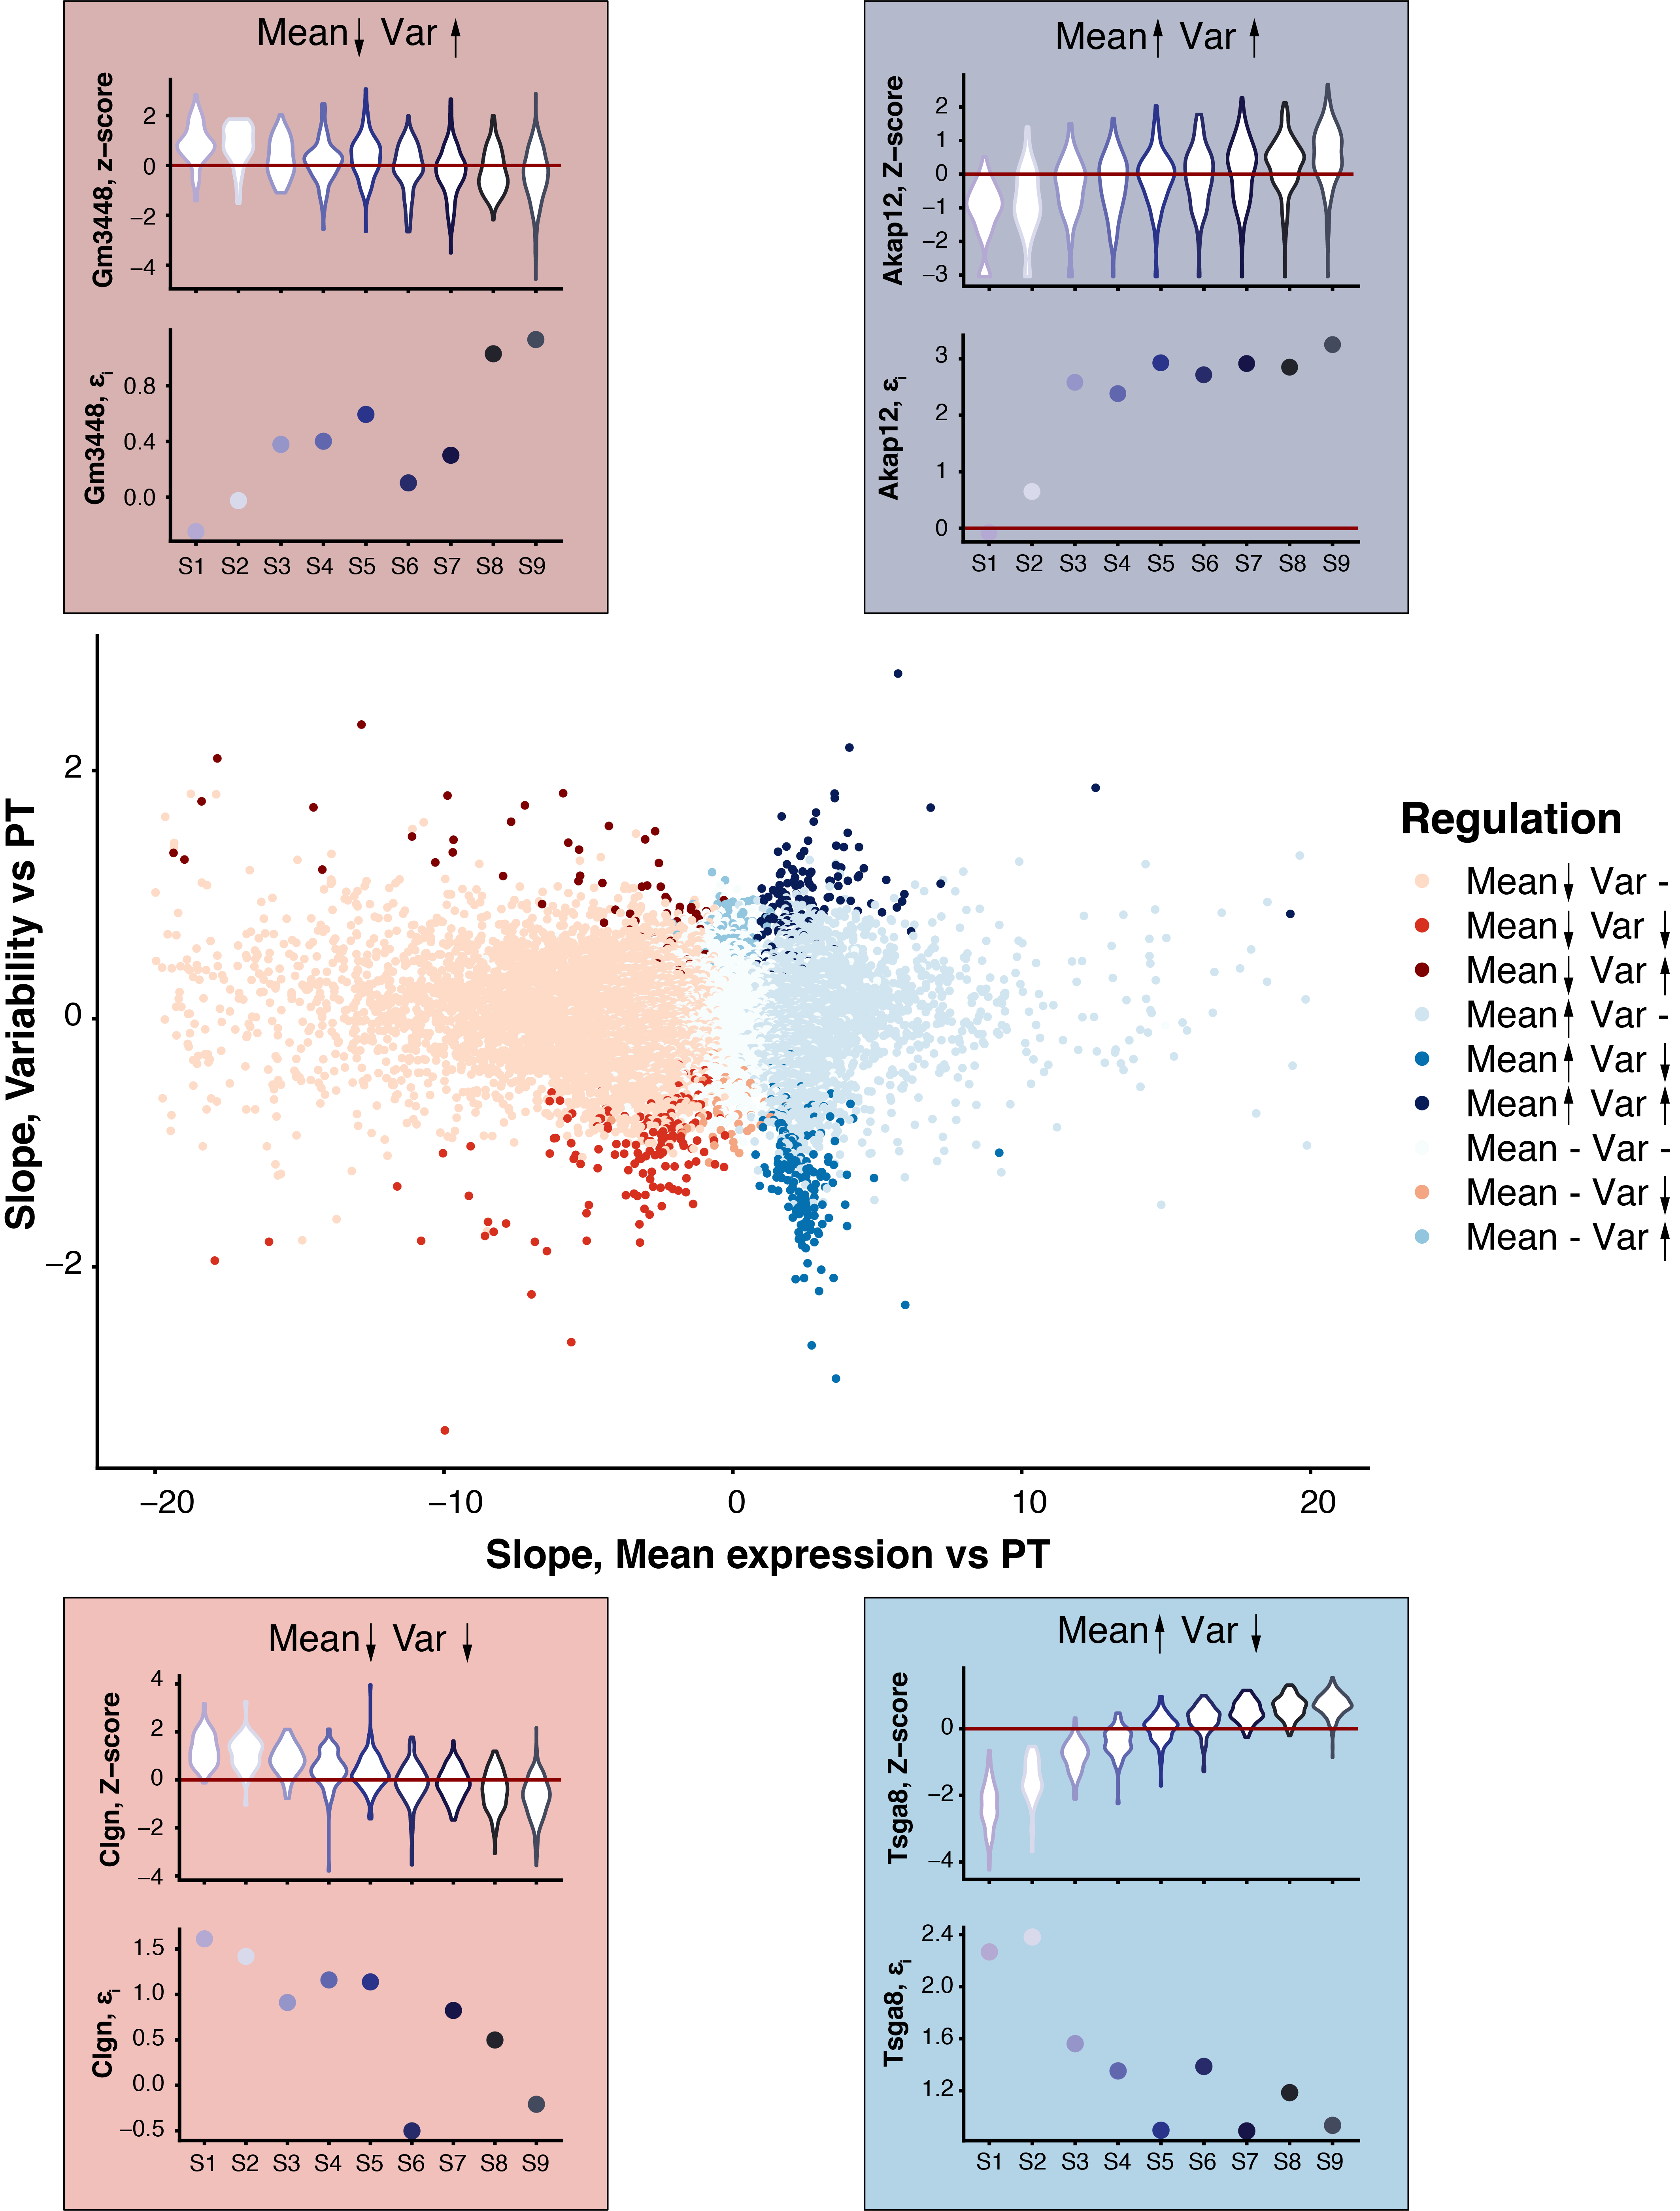
\includegraphics[width=0.8\textwidth]{Fig_15.png}
\caption[Increased expression variability during ageing in different CD4$^+$ T cell subsets]{\textbf{Increased expression variability during ageing in different CD4$^+$ T cell subsets.} \\
\textbf{(A)} Thymus and spleen were collected from young and old B6 mice, dissociated into single cell suspensions, stained with viability dye and antibodies against CD4, CD8, CD24 and Qa2 for thymocytes or antibodies against CD4, CD44, CD62L, CD24 and Qa2 for splenocytes. FACS plots shown are gated on single, live cells and either CD4$^+$ CD8$^-$ CD4 single positive (SP) thymocytes (thymus) or CD44$^{lo}$ CD62L$^{hi}$ naive CD4$^+$ T cells (spleen). Percentages relate to total gated cells. Representative FACS plots of 5 young and 5 old mice are shown. In the thymus the majority of CD4 SP express markers of recent thymic emigrants (RTEs, CD24hi Qa2lo) while in the spleen naive CD4$^+$ T cells are comprised mainly of mature naive cells (red box); \textbf{(B)} Analysis of flow cytometry data from (A). Significance of difference was calculated by Mann-Whitney test (ns = not significant); \textbf{(C)} Spleen were collected from young and old B6 mice, dissociated into single cell suspensions, stained with viability dye and antibodies against CD4, CD44, CD62L, CD24, Qa2, CD69, and PD-1. FACS plots were gated on single, live, CD4$^+$ T cells and subsequently on either CD44$^{lo}$ CD62L$^{hi}$ (Naive) or CD44$^{hi}$ CD62L$^{lo}$ (Effector Memory, EM) subsets. Expression of CD69 and PD-1 was analysed in these subsets. Results shown are pooled from 10 independent experiments with spleens harvested from 5 young and 5 old mice. Significance of difference was calculated by two-way ANOVA ($^{\ast{}\ast}$p $\leq$ 0.01; $^{\ast{}\ast{}\ast{}\ast}$p $\leq$ 0.0001); \textbf{(D)} Activated, FACS-purified naive CD4$^+$ T cells from old animals showed higher transcriptional variability compared to young animals; \textbf{(E)} Activated, FACS-purified effector memory CD4$^+$ T cells from old animals showed higher transcriptional variability compared to young animals.}
\label{fig1:EM_Naive_CD4}
\end{figure}

An additional confounding factor when quantifying expression variability in aged CD4$^+$ T cells could be the presence of recent thymic emigrants (RTEs). Thymic output and maturation of RTEs contributes significantly to the maintenance of the naive CD4$^+$ T cell pool in the periphery and is affected by aging \citep{Boursalian2004, Hale2006, Fink2013}. To exclude different proportions of RTEs within the naive CD4$^+$ T cell pool, we characterized CD4 single positive (SP) thymocytes and splenic naive CD4$^+$ T cell by flow cytometry using CD24 and Qa2 – a marker combination used for identification of RTEs in peripheral tissues \citep{Boursalian2004, Hale2006}. The majority of CD4 SP thymocytes showed a CD24$^{hi}$ Qa2$^{lo}$ phenotype \textbf{(Fig. \ref{fig1:EM_Naive_CD4}A)}. In contrast, we detected only a very small population of RTEs (CD24hi Qa2lo, ~2\%) within splenic naive CD4$^+$ T cell pool of young and old mice \textbf{(Fig. \ref{fig1:EM_Naive_CD4}A and B)} \citep{Hale2006}, suggesting minimal contamination of RTEs in naive CD4$^+$ T cells purified by MACS.\\

Next, we examined whether the age-mediated increase in cell-to-cell variability is conserved across different memory subsets of CD4$^+$ T cells. As expected, a significantly higher proportion of effector memory CD4$^+$ T cells in old animals expressed the activation markers CD69 and PD-1, indicating that a larger fraction of cells is already in an activated state \textbf{(Fig. \ref{fig1:EM_Naive_CD4}C)}. To avoid interference in cell-to-cell variability by endogenously activated cells, cells stained positive for CD69 and/or PD-1 were excluded during the sort of effector memory CD4$^+$ T cells by FACS. Critically, the core activation genes showed an increase in variability in older animals in both naive and effector memory CD4$^+$ T cell subsets \textbf{(Fig. \ref{fig1:EM_Naive_CD4}D and E)}.\\

To conclude, ageing reduces the fraction of cells in which immune activation genes are up-regulated, thus increasing cell-to-cell heterogeneity and attenuating the response to stimulation across multiple CD4$^+$ T cell subsets.

\newpage

\section{Discussion}

How cell-type-specific gene expression programs change during organismal lifespan has long been debated \citep{Bahar2006, Warren2007} but few studies in mammals have quantified the cell-to-cell transcriptome-wide differences that accumulate during aging \citep{Kowalczyk2015}. Here, we systematically explored the effect of aging on the dynamic activation program of primary naive CD4$^+$ T cells in two sub-species of mice as a powerful, well-characterized, and versatile model system \citep{Shay2013}. With this system, we could discriminate the intrinsic effects of ageing from changes due to pathogen-induced immune activation by using mice housed in specific pathogen-free barrier facilities for experiments \citep{Beura2016}.\\

By activating naive CD4$^+$ T cells and quantifying the transcriptional responses of hundreds of single-cells using scRNA-Seq, we confirmed that translation processes and immune response genes are rapidly up-regulated \citep{Neme2016, Asmal2003}. We newly discovered that cell-to-cell variability is simultaneously reduced across thousands of transcripts that do not show changes in gene expression levels. In other words, immune activation rapidly reduces transcriptional heterogeneity across the otherwise-diverse population of CD4$^+$ T cells, revealing a regulatory strategy identical to how iPS reprogramming dynamically restructures transcriptional programs \citep{Buganim2012}. \\

Comparison of gene expression levels across species have been used as a means to identify transcription under strong selection in tissues \citep{Brawand2011, Sudmant2015, Romero2012, Barbosa-Morais2012, Perry2012}, including bulk CD4$^+$ T cells from young mice and humans during immune stimulation \citep{Shay2013}. As expected, we identified a common set of activation genes, including \textit{Il2ra}, that are up-regulated across sub-species; in addition, our scRNA-Seq analyses newly revealed that immune stimulation results in the vast majority of cells within each species up-regulating these genes. In contrast, we discovered that genes whose mean expression was up-regulated in a species-specific manner were often activated in only a small fraction of cells, suggesting weaker selection. Indeed, species-specific up-regulated genes showed no functional enrichment. This discovery suggests a novel defining feature of functional target genes: coherent transcriptional up-regulation across a population of cells. \\

Many attempts have been made to identify transcriptional signatures associated with ageing \citep{Magalhaes2009, Chen2013, Kowalczyk2015}. On a genome-wide basis, we observed that ageing has minimal effects on mean expression levels in unstimulated and stimulated CD4$^+$ T cells. However, in the core set of activated genes, in both species and in distinct CD$^+$ T cell subsets we found a markedly more heterogeneous transcriptional response to stimulation in older mice. Indeed, this increased heterogeneity was driven by ageing associated differences in the reduced fraction of cells across the population that fully responded to stimulation. High numbers of CD4$^+$ T cells are needed to combat infection and cancer. The discovery that CD4$^+$ T cells from aged mice are unable to up-regulate a core activation program robustly may in part explain the decrease of immune function observed in aged mammals \citep{Goronzy2013}. More generally, in the context of the current understanding of transcriptional dysregulation and chromatin destabilization during aging \citep{Booth2016}, increased cell-to-cell transcriptional variability is a major, and largely unexplored, intrinsic factor.\\

\todo{Discuss Stephen Quakes paper and epiCytof and expand on other relevant papers.}

\todo{Discuss tissue specificity.}



